\documentclass{elsarticle}
\usepackage{placeins}
\usepackage{amsmath}
\usepackage{amssymb}
\usepackage{graphicx}
\usepackage{subcaption}
\usepackage{lineno}
\usepackage{xcolor}
\usepackage{colortbl}
\usepackage{adjustbox}
\usepackage{multirow}
\usepackage{lscape}
\usepackage{multicol}
\usepackage{wrapfig}
\usepackage{float}
\usepackage{xparse}
\usepackage{dblfloatfix}
\usepackage[T1]{fontenc}
\usepackage[utf8]{inputenc}
\usepackage{lmodern}
\usepackage[margin=0.78in]{geometry}
\usepackage{microtype}
\usepackage{booktabs}
\usepackage{longtable}
\usepackage{caption}
\usepackage[hidelinks]{hyperref}

\captionsetup{font=small,labelfont=bf}

\setlength{\textfloatsep}{10pt plus 2pt minus 2pt}
\setlength{\floatsep}{8pt plus 2pt minus 2pt}
\setlength{\intextsep}{8pt plus 2pt minus 2pt}
\setlength{\columnsep}{1cm}

\NewDocumentCommand{\evalat}{sO{\big}mm}{%
	\IfBooleanTF{#1}
	{\left. #3 \right|_{#4}}
	{#3#2|_{#4}}%
}

\DeclareMathOperator*{\argmax}{arg\,max}
\DeclareMathOperator*{\argmin}{arg\,min}

\modulolinenumbers[5]

\DeclareGraphicsExtensions{.png,.pdf}
\usepackage{natbib}
\bibliographystyle{elsarticle-num}


\journal{...}
%-----------------------------------------------------
\begin{document}
%-------------------------------------------
\begin{titlepage}
	\begin{center}
		
		\vspace*{1cm}
		
		\textbf{A Robust Gradient Estimation Framework for Noise-Resistant HOG Feature Extraction}
		
		\vspace{1cm}
		
		Ali Mehrizi$^{a}$, Hadi Sadoghi Yazdi$^{a,b,*}$
		
		\vspace{0.7cm}
		
		$^{a}$Department of Computer Engineering, Ferdowsi University of Mashhad,
		Mashhad, Iran
		
		$^{b}$Center of Excellence on Soft Computing and Intelligent Information Processing,
		Ferdowsi University of Mashhad, Mashhad, Iran
		
	\end{center}
	
	\vspace{0.5cm}
	
	Email-addresses:
	
	Ali Mehrizi (mehrizi.a@gmail.com),
	
	Hadi Sadoghi Yazdi (h-sadoghi@um.ac.ir)
	
	\vspace{0.3cm}
	
	$^{*}$Corresponding author
	
\end{titlepage}
%-------------------------------------------
\begin{frontmatter}
%\title{Robust Histogram of Oriented Gradient}
%--------------------------------------------------
%\author[mythirdaryaddress,mysecondaryaddress]{Masoud Akhgar}
%\ead{Masoudmdar78@gmail.com}

%\author[mymainaddress,mysecondaryaddress]{Tahereh Bahraini}
%\ead{bahraini.tahereh@mail.um.ac.ir}

%\author[mysecondaryaddress,mythirdaryaddress]{Hadi Sadoghi Yazdi\corref{mycorrespondingauthor}}
%\cortext[mycorrespondingauthor]{Corresponding author}
%\ead{h-sadoghi@um.ac.ir}

%\address[mainaddressRS]{Department of Civil Engineering, Ferdowsi University of Mashhad, Mashhad, Iran}
%\address[mysecondaryaddress]{Center of Excellence on Soft Computing and Intelligent Information Processing, Ferdowsi University of Mashhad, Mashhad, Iran}
%\address[mymainaddress]{Department of Electrical Engineering, Ferdowsi University of Mashhad, Mashhad, Iran}
%\address[mythirdaryaddress]{Department of Computer Engineering, Ferdowsi University of Mashhad, Mashhad, Iran}
%-----------------------------------------------------
%-----------------------------------------------------
\begin{abstract}
	
	Histogram of Oriented Gradients (HOG) is a widely used feature descriptor
	in computer vision applications; however, its dependence on image gradients
	makes it sensitive to noise contamination. In this work, a robust gradient
	estimation framework is proposed to improve the stability of HOG features
	under noisy conditions. The proposed framework replaces the conventional
	gradient computation stage of HOG with Taylor-series-based local gradient
	estimators combined with robust optimization strategies.
	
	Three formulations are investigated, including direct squared-loss,
	iterative squared-loss, and correntropy-based estimators. The first method
	provides a computationally efficient approximation, while the iterative and
	correntropy formulations improve gradient stability by optimizing the local
	estimation process and reducing the influence of outlier pixels,
	respectively. Extensive experiments are conducted under noise-free,
	Gaussian, and salt-and-pepper noise conditions, and the resulting HOG
	representations are compared with the conventional Sobel-based approach.
	
	The results demonstrate that the proposed estimators preserve the main image
	structures in clean conditions and provide improved robustness under noisy
	observations, particularly for impulsive salt-and-pepper noise. The
	correntropy-based formulation achieves the highest robustness among the
	evaluated methods at the cost of increased computational complexity. These
	findings indicate that the proposed framework provides an effective
	trade-off between HOG stability and computational efficiency for noisy image
	feature extraction.
	
\end{abstract}
%------------------------------------------------
\begin{keyword}
	Histogram of Oriented Gradients (HOG), 
	Gradient estimation, 
	Noise-resistant feature extraction, 
	Robust optimization, 
	Correntropy loss
\end{keyword}
%------------------------------------------------
\end{frontmatter}
\linenumbers
%------------------------------------------------
\section{Introduction}

Histogram of Oriented Gradients (HOG) is one of the most widely used feature descriptors in computer vision, introduced by Dalal and Triggs \cite{H1}. HOG extracts discriminative features by computing local image gradients, normalizing their magnitudes, and constructing orientation histograms. Due to its balance between computational complexity and recognition accuracy, HOG-based approaches have been extensively applied in various tasks, including texture classification \cite{H2}, face recognition \cite{H3,H4}, human activity recognition \cite{H6}, and vehicle detection \cite{H7}. Moreover, combining HOG features with classifiers such as Adaboost \cite{H8} and Support Vector Machines \cite{H9,H10} has resulted in effective object detection frameworks.

Several studies have attempted to improve the performance of HOG descriptors by modifying feature representations, incorporating multi-scale information, or combining HOG with complementary features. For example, different feature fusion strategies have been investigated for pedestrian detection \cite{H23,H24,H25,H26,H27}. Multi-scale HOG representations have also been explored to improve detection performance \cite{H16,H17}. Furthermore, dimensionality reduction and classification-based frameworks have been employed to enhance the efficiency of HOG-based systems \cite{H18,H19}. Other studies have focused on accelerating HOG computation and reducing its computational cost \cite{H13,H14,H15,H22}.

Despite these improvements, most existing approaches focus on modifying the descriptor representation or the subsequent classification stage, while the fundamental gradient estimation step of HOG has received comparatively less attention. Since HOG features are directly generated from image gradients, errors introduced during gradient computation can significantly affect the final descriptor, particularly when images are contaminated by noise. Conventional gradient operators, such as Sobel-based estimation, are sensitive to both Gaussian and impulsive noises, which may lead to inaccurate edge representation and degraded HOG performance.

In this work, we address this limitation by proposing a robust gradient estimation framework for noise-resistant HOG feature extraction. The proposed framework replaces conventional gradient operators in the HOG computation pipeline and investigates three estimation strategies with different robustness-complexity trade-offs. First, a direct least-squares formulation provides an efficient non-iterative gradient estimator. Then, an iterative least-squares optimization is introduced to refine the estimation accuracy. Finally, a correntropy-based formulation is employed to improve robustness against outlier noises. The main contributions of this paper are summarized as follows:

\begin{itemize}
	\item A Taylor-based local gradient estimation framework is introduced to improve the robustness of HOG feature extraction against image noise.
	\item Three gradient estimation strategies, including direct squared-loss, iterative squared-loss, and correntropy-based optimization, are investigated to provide different accuracy and computational cost trade-offs.
	\item The proposed framework is evaluated under clean, Gaussian, and salt-and-pepper noise conditions and compared with the conventional Sobel gradient operator.
\end{itemize}

The remainder of this paper is organized as follows. Section 2 introduces the background concepts, including image gradients and HOG feature extraction. Section 3 presents the proposed robust gradient estimation framework. Experimental results are discussed in Section 4, and conclusions are provided in Section 5. 
%----------------------------------------------------
\section{Background}

\subsection{Image and Gradient Representation}

Let $ f : \mathbb{R}^2 \rightarrow \mathbb{R} $ denote a grayscale image intensity function. Local structural information in an image can be characterized by its spatial gradient, defined as
\begin{equation}
	\nabla f(x,y) = \left( \frac{\partial f(x,y)}{\partial x}, \frac{\partial f(x,y)}{\partial y} \right).
\end{equation}

The gradient magnitude and orientation are given by
\begin{equation}
	|\nabla f(x,y)| = \sqrt{ \left( \frac{\partial f}{\partial x} \right)^2 + \left( \frac{\partial f}{\partial y} \right)^2 },
\end{equation}
\begin{equation}
	\theta(x,y) = \mathrm{atan2} \left( \frac{\partial f}{\partial y}, \frac{\partial f}{\partial x} \right).
\end{equation}

In digital images, derivatives are approximated using discrete operators. A common approach is the central difference scheme:
\begin{equation}
	\frac{\partial f}{\partial x} \approx \frac{f(x+1,y) - f(x-1,y)}{2}, \quad
	\frac{\partial f}{\partial y} \approx \frac{f(x,y+1) - f(x,y-1)}{2}.
\end{equation}

For improved robustness to noise, convolution-based operators such as Sobel filters are widely used:
\begin{equation}
	S_x =
	\begin{bmatrix}
		-1 & 0 & 1 \
		-2 & 0 & 2 \
		-1 & 0 & 1
	\end{bmatrix}, \quad
	S_y =
	\begin{bmatrix}
		-1 & -2 & -1 \
		0 & 0 & 0 \
		1 & 2 & 1
	\end{bmatrix}.
\end{equation}

\subsection{Histogram of Oriented Gradients (HOG)}

The Histogram of Oriented Gradients (HOG) is a feature descriptor that captures local shape information by encoding the distribution of gradient orientations. The image is divided into small spatial regions called \textit{cells} (typically $8 \times 8$ pixels). For each cell, a histogram over a predefined set of orientation bins is constructed.

Each pixel contributes to the histogram according to its gradient orientation, with a vote weighted by its gradient magnitude. Let $ \mathcal{C} $ denote a cell and $ B_k $ the $k$-th orientation bin. The histogram value for bin $k$ is defined as
\begin{equation}
	h_k = \sum_{(x,y) \in \mathcal{C}} |\nabla f(x,y)| \cdot \delta(\theta(x,y) \in B_k),
\end{equation}
where $ \delta(\cdot) $ is an indicator function that assigns each gradient orientation to its corresponding bin.

An illustrative example of gradient orientations, magnitudes, and their weighted contributions to orientation bins is shown in Fig.~\ref{fig1}.

To improve robustness against illumination and contrast variations, neighboring cells are grouped into larger regions called \textit{blocks}. The concatenated histogram vector within each block is normalized using $L_2$-normalization:
\begin{equation}
	\mathbf{v} \leftarrow \frac{\mathbf{v}}{\sqrt{ |\mathbf{v}|_2^2 + \epsilon^2 }},
\end{equation}
where $ \mathbf{v} $ is the block descriptor and $ \epsilon $ is a small constant for numerical stability.

The final HOG descriptor is obtained by concatenating normalized block descriptors over the entire image.

\begin{figure*}[!t]
	\centering
	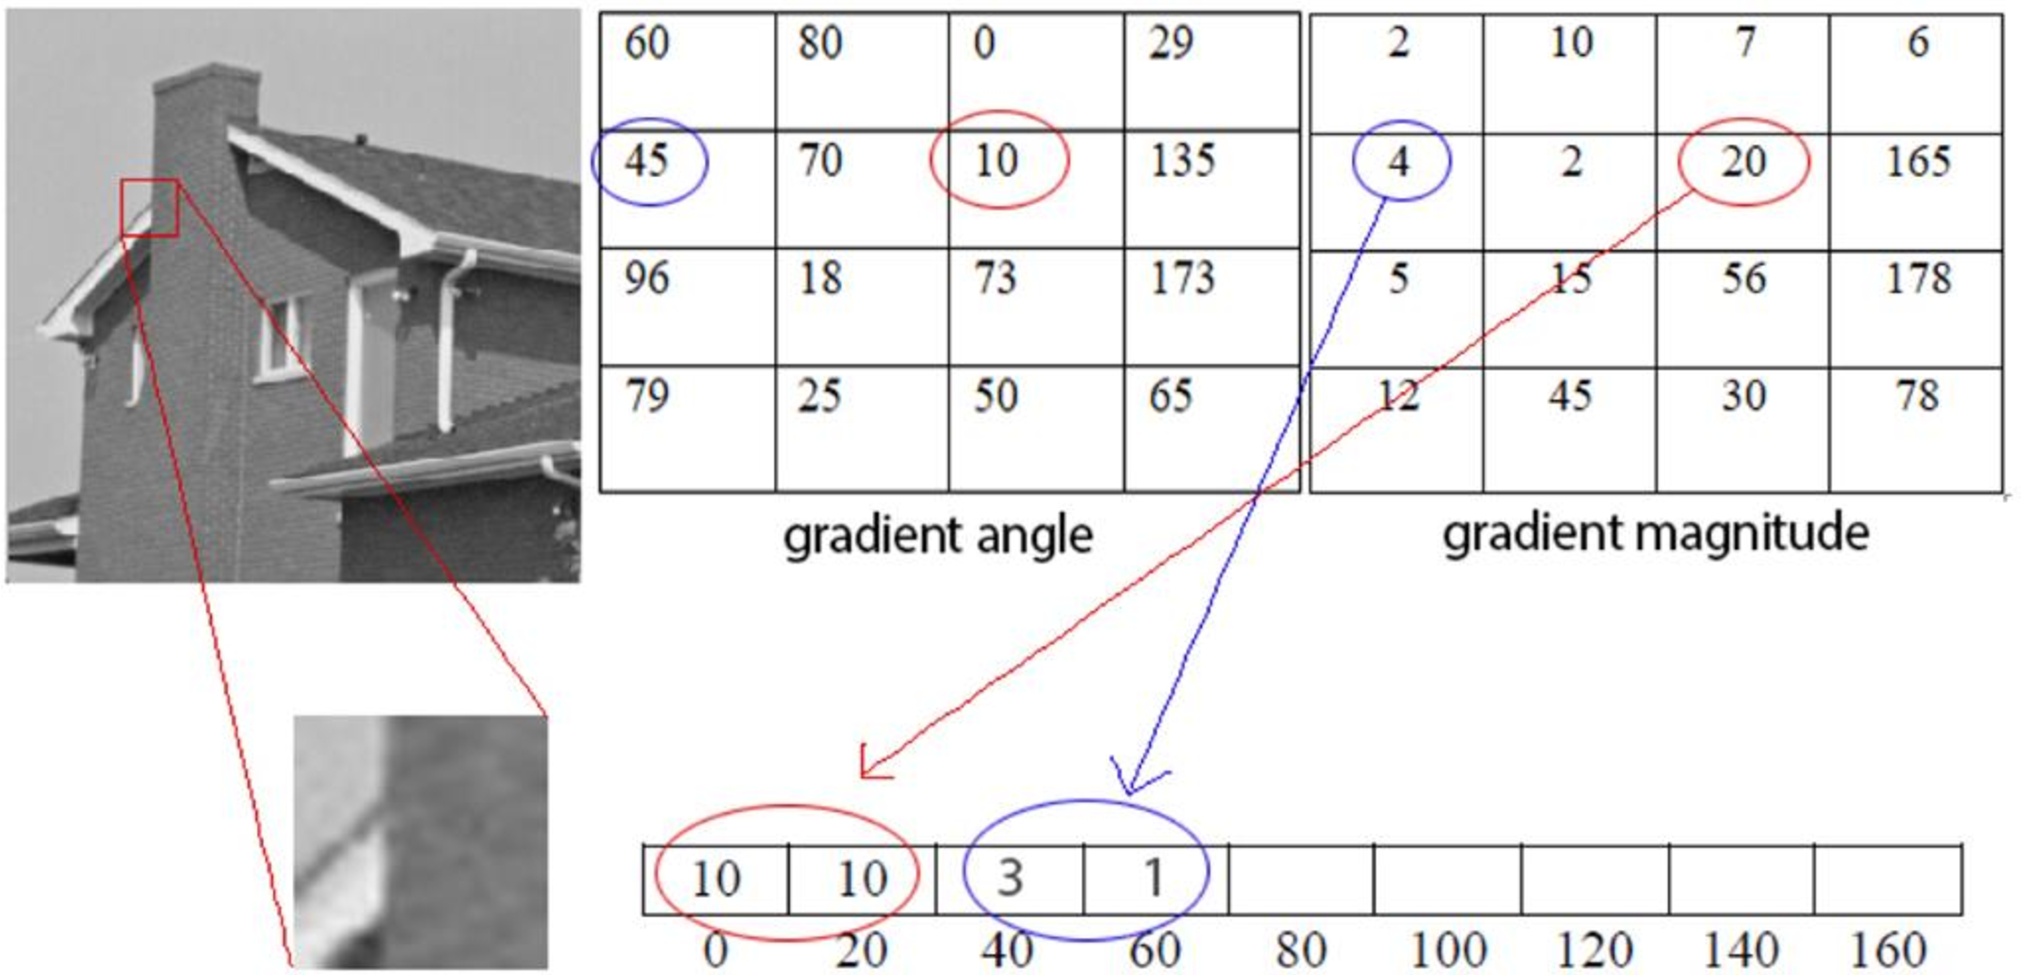
\includegraphics[width=0.75\textwidth]{figures/Drawing1.pdf}
	\caption{Illustration of gradient orientations and magnitudes within a cell, and their weighted voting into orientation bins in the HOG descriptor.}
	\label{fig1}
\end{figure*}

%------------------------------------------------
\section{Proposed Method}

In this section, we present the proposed framework for robust gradient estimation.
While conventional methods such as finite differences and Sobel operators provide efficient approximations,
their performance degrades significantly in the presence of noise and local intensity variations.

To address this limitation, we propose a local modeling approach based on Taylor approximation,
where gradient estimation is formulated as a regression problem within a neighborhood of each pixel.
This formulation enables the incorporation of robust objective functions to reduce the influence of noise and outliers.

The overall pipeline of the proposed method is illustrated in Fig.~\ref{fig2}.
First, a local neighborhood is extracted around each pixel.
Then, a Taylor-based linear model is constructed to describe local intensity variations.
Next, a robust objective function is employed to improve estimation stability.
Finally, the resulting optimization problem is solved to obtain the gradient components.
%-----------------------------------------------------------	
\begin{figure*}[!th]
	\centering
	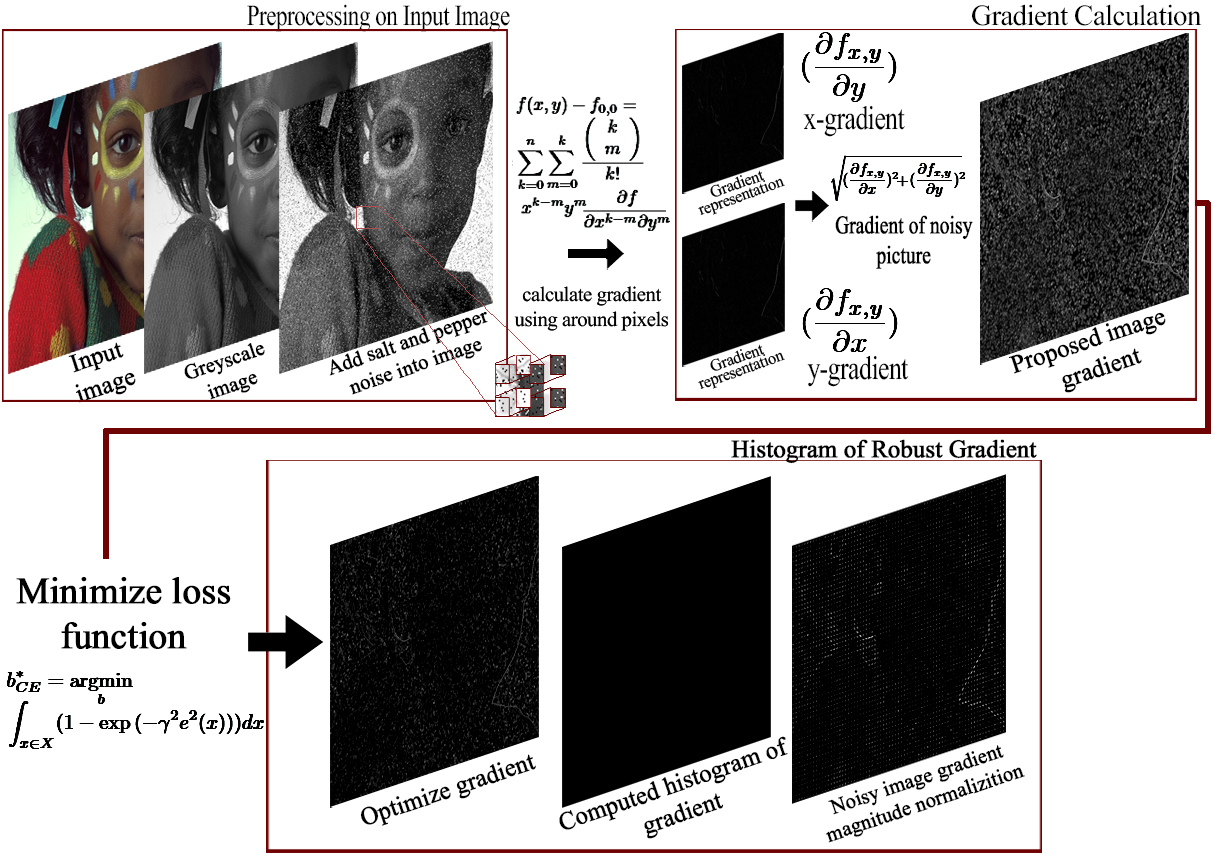
\includegraphics[height=7.5cm,width=13cm]{figures/schematic_final.jpg}
	\caption{The block diagram of the proposed process for the calculating the robust HOG}
	\label{fig2}
\end{figure*}
%-----------------------------------------------------------

The following subsections describe each step in detail.

%----------------------------------------------------------

\subsection{Problem Formulation}
Consider a set of $n$ ordered real points such that $x_1 < x_2 < \cdots < x_n$. Let $f$ be a sufficiently smooth (i.e., continuous and differentiable up to the required order) function defined on the interval $[x_1, x_n]$. 

To approximate local derivatives of the image intensity function, we employ a
Taylor expansion around a local reference point. For each estimation location,
the coordinate system is shifted such that the reference point is considered
as the origin of the local neighborhood. Therefore, the local intensity
variation can be expressed as:

\begin{equation}\label{Q1}
	f(x)=f(0)+f'(0)x+\frac{f''(0)}{2!}x^2+\cdots+
	\frac{f^{(z)}(0)}{z!}x^z+O(x^{z+1}),
\end{equation}

where $O(x^{z+1})$ denotes the truncation error of the Taylor expansion.

By evaluating \eqref{Q1} at symmetric points $x = \pm 1$ and truncating at order $z = 2$, we obtain:
\begin{equation}\label{Q2}
	f'(0) = \frac{f(1) - f(-1)}{2} + O(1),
\end{equation}
which corresponds to the classical central finite-difference approximation.

Since the function values are assumed to be known at discrete sample points, the derivative $f'(0)$ can be estimated numerically. In general, estimating derivatives requires constructing a system of equations obtained from Taylor expansions around zero at multiple sampling locations.

This formulation naturally recovers classical finite-difference schemes. In particular, the Sobel operator can be interpreted as a discrete first-order approximation derived from this framework by restricting the model to a minimal $3 \times 3$ neighborhood and a first-order truncation.

More generally, by evaluating the Taylor expansion at symmetric points around zero, such as $x = \pm 1, \pm 2, \ldots, \pm \frac{n}{2}$, we obtain a system of linear equations in terms of the derivatives of $f$ at the origin. Truncating the series at order $z$ and neglecting higher-order terms yields a solvable linear system for estimating derivatives.

For example, evaluating \eqref{Q1} at selected points gives:
\begin{equation}\label{Q3}
	f(1) = f(0) + f'(0) + \frac{f''(0)}{2!} + \cdots + \frac{f^{(z)}(0)}{z!} + O(1),
\end{equation}

\begin{equation}\label{Q4}
	f(-1) = f(0) - f'(0) + \frac{f''(0)}{2!} + \cdots + (-1)^z \frac{f^{(z)}(0)}{z!} + O(1),
\end{equation}

\begin{equation}\label{Q5}
	f\left(\frac{n}{2}\right) = f(0) + \frac{n}{2} f'(0) + \frac{\left(\frac{n}{2}\right)^2}{2!} f''(0) + \cdots + \frac{\left(\frac{n}{2}\right)^z}{z!} f^{(z)}(0) + O\left(\left(\frac{n}{2}\right)^{z+1}\right),
\end{equation}

\begin{equation}\label{Q6}
	f\left(-\frac{n}{2}\right) = f(0) - \frac{n}{2} f'(0) + \frac{\left(\frac{n}{2}\right)^2}{2!} f''(0) + \cdots + (-1)^z \frac{\left(\frac{n}{2}\right)^z}{z!} f^{(z)}(0) + O\left(\left(\frac{n}{2}\right)^{z+1}\right).
\end{equation}

To estimate derivatives up to order $n$, we truncate the Taylor expansion in \eqref{Q1} at $z = n$. By subtracting $f(0)$ from both sides of the resulting equations, we obtain a linear system that can be written in matrix form. Let $\mathcal{N} = \{x_1, x_2, \dots, x_M\}$ denote the set of sampling points.

\begin{equation}\label{Q9}
	\begin{aligned}
		\mathbf{A}
		\begin{bmatrix}
			f'(0) \\
			f''(0) \\
			\vdots \\
			f^{(n)}(0)
		\end{bmatrix}
		=
		\begin{bmatrix}
			f(x_1)-f(0) \\
			f(x_2)-f(0) \\
			\vdots \\
			f(x_M)-f(0)
		\end{bmatrix},
	\end{aligned}
\end{equation}
where the coefficient matrix $\mathbf{A}$ is defined as:
\[
\mathbf{A} =
\begin{bmatrix}
	x_1 & \frac{x_1^2}{2!} & \cdots & \frac{x_1^n}{n!} \\
	x_2 & \frac{x_2^2}{2!} & \cdots & \frac{x_2^n}{n!} \\
	\vdots & \vdots & \ddots & \vdots \\
	x_M & \frac{x_M^2}{2!} & \cdots & \frac{x_M^n}{n!}
\end{bmatrix}.
\]

Let the $j$-th row of $\mathbf{A}$ be:
\begin{equation}\label{Q7}
	R_j(n) = \begin{bmatrix}
		x_j & \frac{x_j^2}{2!} & \cdots & \frac{x_j^n}{n!}
	\end{bmatrix}.
\end{equation}

Define the derivative vector:
\begin{equation}
	\mathbf{d} =
	\begin{bmatrix}
		f'(0) & f''(0) & \cdots & f^{(n)}(0)
	\end{bmatrix}^T.
\end{equation}

Then each equation can be written compactly as:
\begin{equation}\label{Q8}
	f(x_j) - f(0) = R_j(n)\mathbf{d}.
\end{equation}

Solving \eqref{Q9} yields numerical estimates of derivatives at the reference point. Applying this procedure across all sample locations enables derivative computation over the entire signal.

\subsubsection{Extension to Two-Dimensional Signals}

The formulation can be extended to two-dimensional functions (e.g., images). Let $f(x,y)$ be a smooth function, and denote $f(0,0)$ by $f_{0,0}$. The Taylor expansion around $(0,0)$ is given by:
\begin{equation}\label{Q10}
	\begin{aligned}
		f(x,y) &= f_{0,0} + f_x x + f_y y \\
		&\quad + \frac{1}{2!} \left( f_{xx} x^2 + 2 f_{xy} xy + f_{yy} y^2 \right) \\
		&\quad + \frac{1}{3!} \left( f_{xxx} x^3 + 3 f_{xxy} x^2 y + 3 f_{xyy} x y^2 + f_{yyy} y^3 \right) + \cdots,
	\end{aligned}
\end{equation}
where all derivatives are evaluated at $(0,0)$.

In compact form:
\begin{equation}\label{Q11}
	f(x,y) - f_{0,0} =
	\sum_{k=1}^{\infty} \sum_{m=0}^{k}
	\frac{x^{k-m} y^{m}}{(k-m)!m!}
	\frac{\partial^{k} f}{\partial x^{k-m} \partial y^{m}}.
\end{equation}

By substituting neighboring sample points $(x_i,y_i)$ into \eqref{Q11}, we obtain a linear system:
\begin{equation}\label{Q12}
	\mathbf{B}\mathbf{d}_{2D} =
	\begin{bmatrix}
		f(x_1,y_1)-f_{0,0} \\
		\vdots \\
		f(x_n,y_n)-f_{0,0}
	\end{bmatrix},
\end{equation}
where $\mathbf{B}$ is constructed from monomials of $(x_i,y_i)$ and $\mathbf{d}_{2D}$ contains partial derivatives.

Increasing the number of terms improves accuracy but also increases computational complexity and sensitivity to noise. Near boundaries, where symmetric neighborhoods are unavailable, one-sided approximations must be used. This trade-off is analogous to polynomial fitting: higher-order models provide better approximation but are more sensitive to noise. This formulation also enables the integration of robust estimation techniques, which will be discussed in the next subsection.

We consider both the squared loss and a correntropy-induced loss to solve the resulting linear system. The squared loss provides an efficient baseline but is sensitive to outliers. To enhance robustness, we adopt a correntropy-based formulation, which can be interpreted as an adaptive reweighting of the squared loss. Both formulations are retained for comparison. We first present the squared loss and then its correntropy-based extension.

\subsection{Least Squares-Based HOG}

To enhance robustness against noise and truncation errors in the Taylor-based formulation presented in the previous subsection, we reformulate the approximation model by explicitly introducing a residual (bias) term. Specifically, we consider:
\begin{equation}\label{QSM}
	f(x) = \hat{f}(x) + b
\end{equation}
where $\hat{f}(x)$ is a truncated Taylor expansion of $f(x)$ around the reference point $x_0 = 0$, and $b$ represents the residual approximation error, which implicitly captures the neglected higher-order terms, i.e., $b \approx O(x^{z+1})$. Using the Taylor expansion up to order $z$, we have:
\begin{equation}
	\hat{f}(x)=\sum_{n=0}^{z}\frac{f^{(n)}(0)}{n!}x^n
\end{equation}

To estimate the optimal value of $b$, we formulate the following least-squares optimization problem:
\begin{equation}\label{Q14_1}
	b^*_{LS}=\argmin_{b}\int_{x\in X} l(e(x)),dx
\end{equation}
where the residual error is defined as:
\begin{equation}
	e(x)=f(x)-\hat{f}(x)-b
\end{equation}
and $X$ denotes the domain of interest.

By adopting the least-squares loss function $l(e(x)) = e^2(x)$, we obtain:
\begin{equation}\label{Q15_1}
	b^*_{LS}=\argmin_{b}\int_{x\in X}\left(f(x)-\hat{f}(x)-b\right)^2 dx
\end{equation}

We truncate the Taylor expansion up to the fourth order and explicitly parameterize higher-order contributions as:
\begin{equation}\label{Q16_1}
	\hat{f}(x)\approx f(0)+f'(0)x+\frac{f''(0)}{2!}x^2+\alpha_1 x^3+\alpha_2 x^4
\end{equation}
where $\alpha_1$ and $\alpha_2$ model higher-order effects beyond the second derivative.

Substituting \eqref{Q16_1} into the objective function yields:
\begin{equation}\label{Q17_1}
	b^*_{LS}=\argmin_{b}\int_{x\in X}\Big(f(x)-\big[f(0)+f'(0)x+\frac{f''(0)}{2!}x^2+\alpha_1 x^3+\alpha_2 x^4 + b \big]\Big)^2 dx
\end{equation}

By taking the derivative with respect to $b$ and setting it to zero, we obtain:
\begin{equation}\label{Q18_1}
	\int_{x\in X}\Big(f(x)-\hat{f}(x)-b\Big) dx = 0
\end{equation}
which leads to the closed-form solution:
\begin{equation}\label{Q19_1}
	b = \frac{1}{|X|}\int_{x\in X} \big(f(x)-\hat{f}(x)\big),dx
\end{equation}

To estimate the unknown parameters, we define the following sub-problems:

\begin{enumerate}
	
	\item \textbf{$b_{LS}$ sub-problem:}
	\begin{equation}\label{Q20_1}
		b_{LS} \approx f(x)-f(0)-f'(0)x-\frac{f''(0)}{2!}x^2
	\end{equation}
	
	\item \textbf{$f'(0)$ sub-problem:}
	
	In practice, instead of solving the full linear system in \eqref{Q9}, we adopt a computationally efficient approximation:
	\begin{equation}\label{Q22_1}
		f'(0)\approx \frac{f(h)-f(-h)}{2h}
	\end{equation}
	
	\item \textbf{$f''(0)$ sub-problem:}
	\begin{equation}\label{Q23_1}
		f''(0)\approx \frac{f(h)-2f(0)+f(-h)}{h^2}
	\end{equation}
	
	\item \textbf{$\alpha$ sub-problem:}
	
	The higher-order coefficients are estimated via a least-squares formulation:
	\begin{equation}\label{Q21_1}
		\alpha = (A^{T}A)^{-1}A^{T}b
	\end{equation}
	where $\alpha=\begin{bmatrix}\alpha_1 \ \alpha_2\end{bmatrix}$ and the design matrix is defined as:
	\[
	A = \begin{bmatrix} x^3 & x^4 \end{bmatrix}.
	\]
	
\end{enumerate}

The first method provides a non-iterative solution, while the second method iteratively updates the parameters until convergence.

%------------------------------------------
\begin{table}[t]
	\centering
	\caption{Algorithm I: Non-iterative least squares-based HOG}
	\label{my-labelI}
	
	\begin{tabular}{l}
		\hline
		\textbf{Input:} $f(x)$, $h$, $D_x=\{x_i\}_{i=1}^{M}$\\
		\textbf{Output:} $f'(x)$ and $f''(x)$\\
		\hline
		\textbf{1:} Estimate $f'(x)$ using \eqref{Q22_1}\\
		\textbf{2:} Estimate $f''(x)$ using \eqref{Q23_1}\\
		\hline
	\end{tabular}
	
\end{table}


%------------------------------------------
\begin{table}[t]
	\centering
	\caption{Algorithm II: Iterative least squares-based HOG}
	\label{my-labelII}
	
	\begin{tabular}{l}
		\hline
		\textbf{Input:} $f(x)$, $h$, $D_x=\{x_i\}_{i=1}^{M}$\\
		\textbf{Output:} $f'(x)$ and $f''(x)$\\
		\textbf{Initialization:} Initialize $b$, $\alpha$, $f'(x)$, $f''(x)$\\
		\hline
		\textbf{Repeat until convergence:}\\
		\textbf{1:} Update $b$ using \eqref{Q20_1}\\
		\textbf{2:} Update $f'(x)$ using \eqref{Q22_1}\\
		\textbf{3:} Update $f''(x)$ using \eqref{Q23_1}\\
		\textbf{4:} Update $\alpha$ using \eqref{Q21_1}\\
		\hline
	\end{tabular}
	
\end{table}
%------------------------------------------

%------------------------------------------------
\subsection{Correntropy-Based Robust Formulation}

The conventional squared loss is highly sensitive to outliers, since large deviations can dominate the optimization process. To enhance robustness, we adopt a correntropy-based loss function, which effectively suppresses the influence of large errors.

The correntropy-induced loss is defined as
\begin{equation}
	l(e(x)) = 1 - \exp\big(-\gamma^2 e^2(x)\big),
\end{equation}
where $e(x)$ denotes the approximation error.

Accordingly, the parameter estimation problem is formulated as
\begin{equation}\label{Q24_1_new}
	b^*_{CE} =
	\argmin_{b}
	\int_{x \in X}
	\left(1 - \exp\big(-\gamma^2 e^2(x)\big)\right)\, dx.
\end{equation}

Since the constant term does not affect the solution, \eqref{Q24_1_new} is equivalent to
\begin{equation}\label{Q25_1_new}
	b^*_{CE} =
	\argmax_{b}
	\int_{x \in X}
	\exp\big(-\gamma^2 e^2(x)\big)\, dx.
\end{equation}

To solve \eqref{Q25_1_new}, we employ the half-quadratic (HQ) optimization framework using the conjugate representation
\begin{equation}\label{Q26_1_new}
	\exp\big(-\gamma^2 e^2(x)\big) =
	\sup_{p(x) < 0}
	\left\{
	\gamma^2 e^2(x)\, p(x) - \Phi\big(p(x)\big)
	\right\},
\end{equation}
where
\begin{equation}
	\Phi(p) = -p \log(-p) + p.
\end{equation}

Substituting \eqref{Q26_1_new} into \eqref{Q25_1_new} leads to the joint optimization problem
\begin{equation}\label{Q28_1_new}
	\{b^*_{CE}, p^*(x)\} =
	\argmax_{b,\, p(x)}
	\int_{x \in X}
	\left(
	\gamma^2 e^2(x)p(x) - \Phi(p(x))
	\right)\, dx.
\end{equation}

This problem can be efficiently solved via alternating optimization. Specifically, fixing $p(x)$ reduces the problem to a weighted least-squares form:
\begin{equation}\label{Q29_1_new}
	b^*_{CE} =
	\argmin_{b}
	\int_{x \in X}
	\big(-p(x)\big)\, e^2(x) \, dx,
\end{equation}
where $-p(x) > 0$ acts as an adaptive weight.

Using a second-order Taylor expansion around $a$, the approximation error can be expressed as
\begin{equation}\label{Q30_1_new}
	e(x) \approx
	f(x) - f(a)
	- f'(a)(x-a)
	- \frac{f''(a)}{2}(x-a)^2.
\end{equation}

By substituting \eqref{Q30_1_new} into \eqref{Q29_1_new}, we obtain a weighted least-squares problem, from which the parameter vector $\boldsymbol{\beta}$ is estimated as
\begin{equation}\label{Q30_2_new}
	\boldsymbol{\beta} =
	(B^T W B)^{-1} B^T W \mathbf{b},
\end{equation}
where $W = \mathrm{diag}(-p(x_i))$ is the diagonal weight matrix.

The first- and second-order derivatives are then computed as
\begin{equation}\label{Q30_3_new}
	f'(0) =
	\frac{1}{2}
	\Big[
	f(1) - f(-1)
	+ \mathbf{z}(-1)\boldsymbol{\beta}
	-
	\mathbf{z}(1)\boldsymbol{\beta}
	\Big],
\end{equation}

\begin{equation}\label{Q30_4_new}
	f''(0) =
	2\Big[
	f(1) - f(0)
	+ \mathbf{z}(1)\boldsymbol{\beta}
	- f'(0)
	\Big],
\end{equation}
where
\begin{equation}
	\mathbf{z}(x) =
	\begin{bmatrix}
		x^3 & x^4
	\end{bmatrix},
	\quad
	\boldsymbol{\beta} =
	\begin{bmatrix}
		\beta_1 \\
		\beta_2
	\end{bmatrix}.
\end{equation}

Next, fixing $b_{CE}$, the auxiliary variable is updated by solving
\begin{equation}\label{Q31_1_new}
	p^*(x) =
	\argmax_{p(x)}
	\left(
	\gamma^2 e^2(x)p(x) - \Phi(p(x))
	\right),
\end{equation}
which yields the closed-form solution
\begin{equation}\label{Q32_1_new}
	p^*(x) = -\exp\big(-\gamma^2 e^2(x)\big).
\end{equation}

Therefore, $p(x)$ acts as an adaptive weight that automatically down-weights large errors, improving robustness against outliers.

The overall correntropy-based iterative procedure is given next.

\begin{table}[t]
	\centering
	\normalsize
	\caption{Proposed Iterative Robust HOG based on Correntropy}
	\label{tab:robust_hog}
	\begin{tabular}{l}
		\hline
		\textbf{Input:} $f(x)$, $D_x = \{x_i\}_{i=1}^M$, $\gamma^2$ \\ 
		\textbf{Output:} $f'(x)$, $f''(x)$ \\
		
		\textbf{Initialize:} $\boldsymbol{\beta}$, $p(x)$ \\
		
		1: Compute $B$ \\
		2: \textbf{repeat} \\
		3: \quad Compute $W = \mathrm{diag}(-p(x_i))$ \\
		4: \quad Update $\boldsymbol{\beta}$ using \eqref{Q30_2_new} \\
		5: \quad Compute $e(x)$ using \eqref{Q30_1_new} \\
		6: \quad Update $p(x)$ using \eqref{Q32_1_new} \\
		7: \textbf{until convergence} \\
		\hline
	\end{tabular}
\end{table}

Repeated iterations may introduce numerical round-off errors due to matrix inversion. Therefore, the number of iterations should be properly controlled to ensure stable convergence and accurate estimation.



\section{Experimental Results}

In this section, a comprehensive experimental evaluation is conducted to assess the effectiveness of the proposed methods for HOG feature extraction under both noise-free and noisy conditions. The experiments are designed to validate the proposed framework from different perspectives, including the accuracy of derivative estimation, the influence of algorithmic parameters, robustness against image degradation, and comparison with conventional edge detection approaches.

The experimental evaluation consists of several stages. First, synthetic functions with known analytical derivatives are employed to validate the correctness and convergence behavior of the proposed derivative estimation framework. Then, the effect of the main parameters and computational complexity of the proposed methods are investigated. Finally, the proposed approaches are evaluated on real-world images under different noise conditions and compared with the Sobel operator as a representative conventional method.

All experiments are performed under identical computational conditions for all compared methods to ensure a fair evaluation. The detailed description of datasets, noise generation procedures, and implementation settings is provided in the following subsection.

To evaluate robustness against image degradation, two common noise types, namely Gaussian and salt-and-pepper noise, are added to the original images at different intensity levels, generating multiple degraded versions of each image. Gaussian noise is generated by sampling from a zero-mean normal distribution with different variance levels, whereas salt-and-pepper noise is introduced by randomly replacing a proportion of pixels with the minimum or maximum intensity values. The noise levels are selected to evaluate the performance of the proposed methods under different degradation scenarios.

All methods, including the proposed approaches and the Sobel operator as a baseline, are implemented in Python and executed under identical computational conditions to ensure a fair comparison. The experiments analyze the effectiveness of the proposed methods under various noise conditions and investigate the influence of key parameters, particularly the neighborhood size parameter $h$, on the quality of HOG extraction.

For visual comparison, the original images and their noisy counterparts are presented in Fig.~\ref{fig:dataset_noise}, enabling a direct qualitative assessment of the effect of noise and the robustness of the evaluated methods.

\FloatBarrier
\begin{figure*}[!t]
	\centering
	
	\begin{subfigure}{\textwidth}
		\centering
		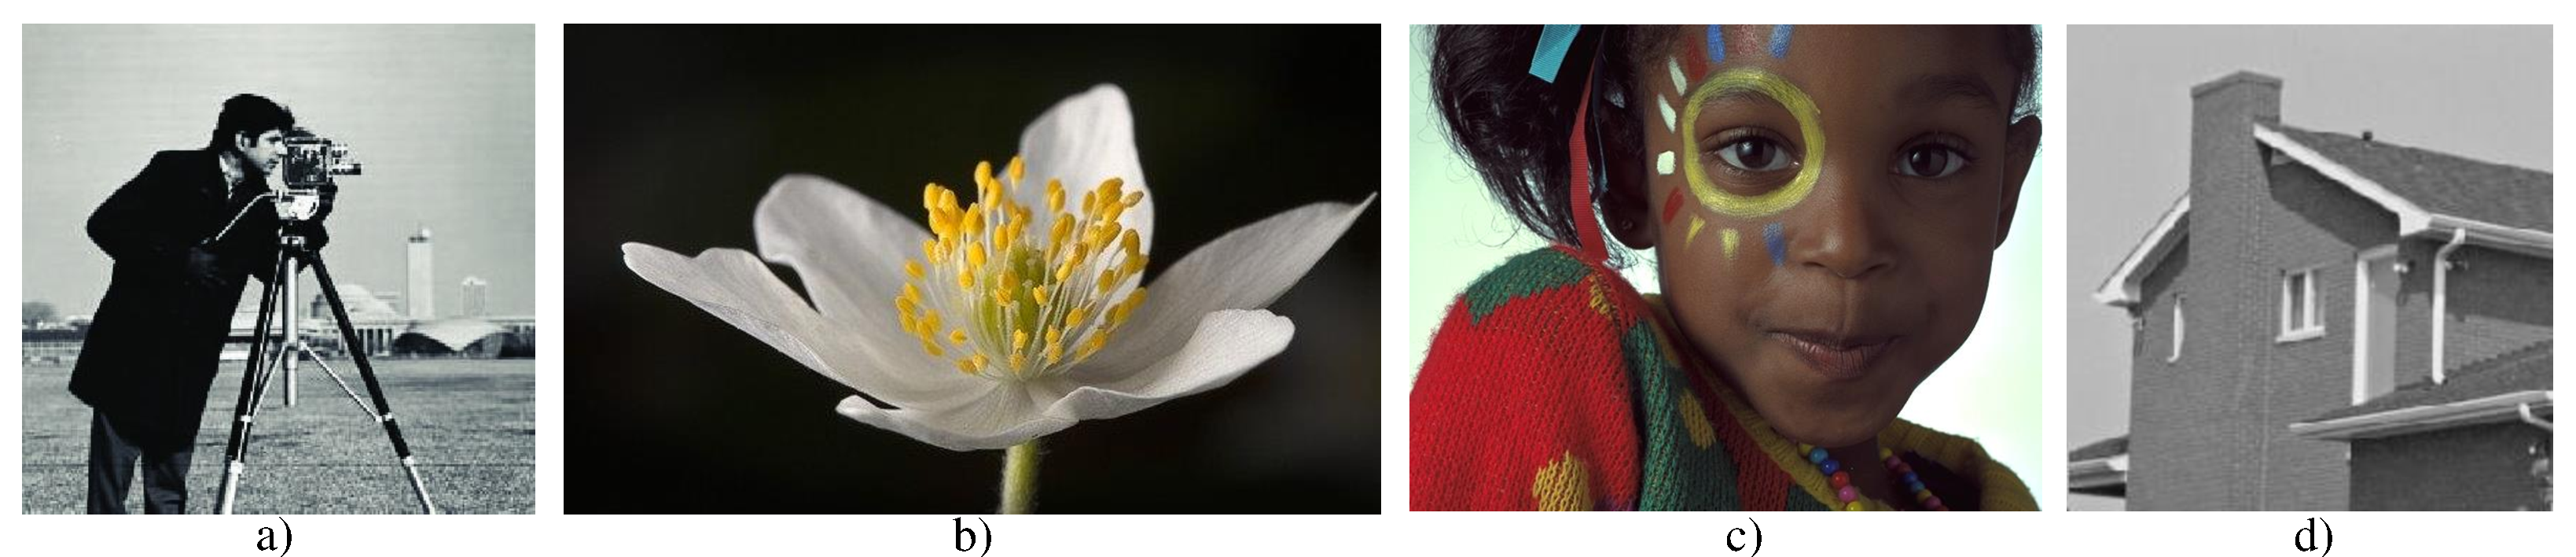
\includegraphics[width=\textwidth]{figures/initial_images1.pdf}
		\caption{Original images}
	\end{subfigure}
	
	\vspace{2mm}
	
	\begin{subfigure}{\textwidth}
		\centering
		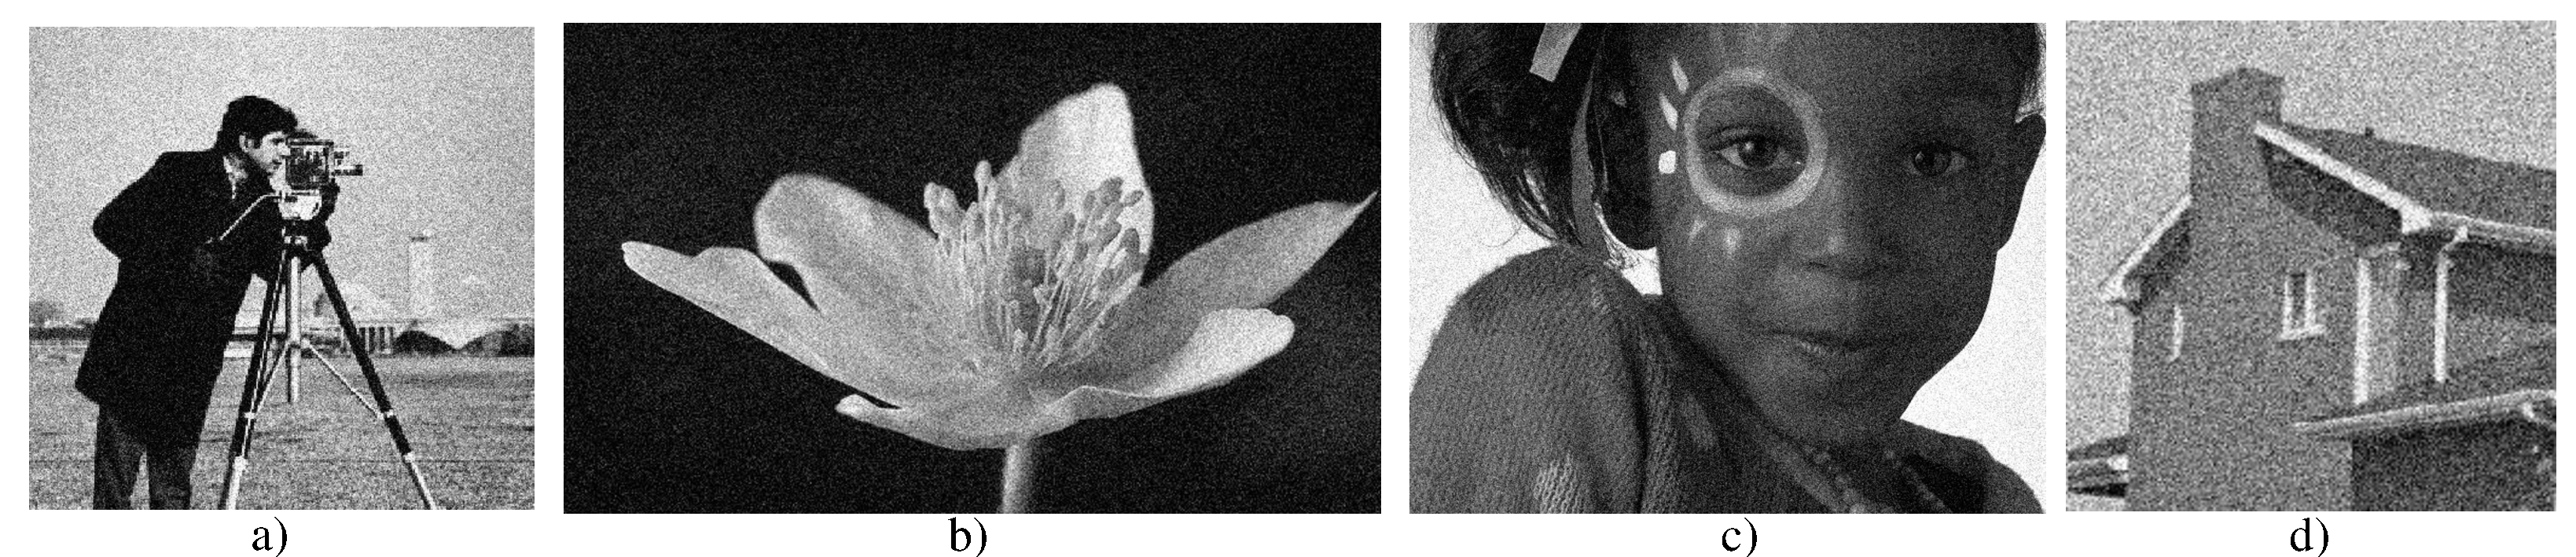
\includegraphics[width=\textwidth]{figures/initial_images2.pdf}
		\caption{Images corrupted with Gaussian noise}
	\end{subfigure}
	
	\vspace{2mm}
	
	\begin{subfigure}{\textwidth}
		\centering
		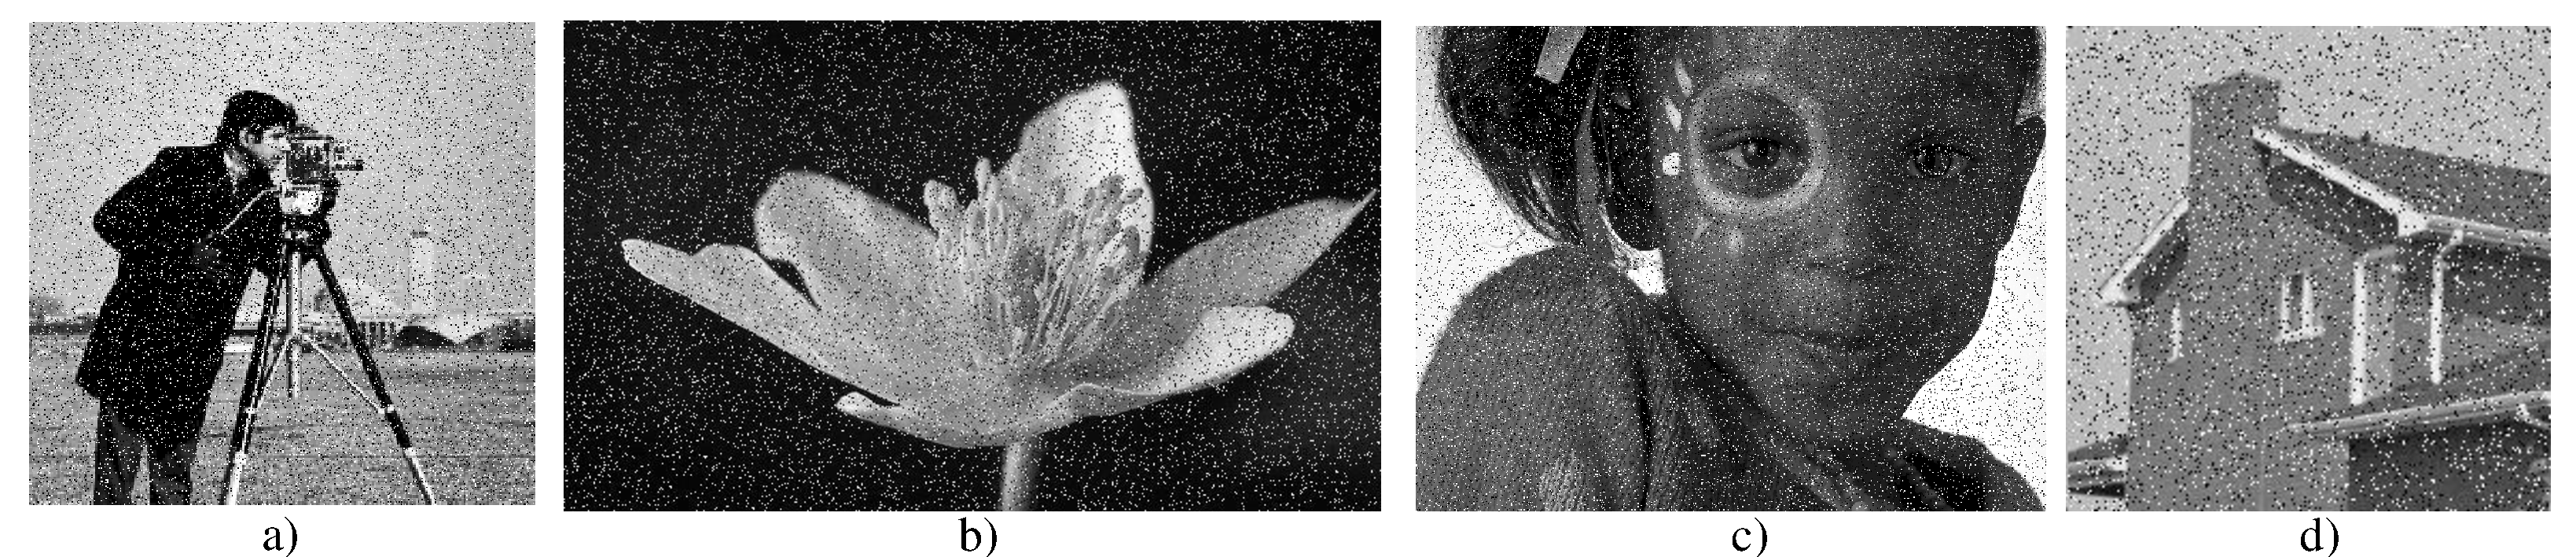
\includegraphics[width=\textwidth]{figures/initial_images3.pdf}
		\caption{Images corrupted with salt-and-pepper noise}
	\end{subfigure}
	
	\caption{Visual comparison of the original images and their degraded versions under different noise conditions. From top to bottom: original images, images corrupted with Gaussian noise, and images corrupted with salt-and-pepper noise.}
	
	\label{fig:dataset_noise}
\end{figure*}
\FloatBarrier

%-----------------------------------------------------------
\FloatBarrier
\subsection{Synthetic-Function Evaluation}
To examine the numerical behavior of the proposed estimators, the synthetic function $f(x,y)=\exp(x+y)$ is considered. Its first-order partial derivatives satisfy $\partial f/\partial x=\partial f/\partial y=\exp(x+y)$ and therefore equal
one at the reference point $(0,0)$. This analytical value provides a reference for assessing the numerical derivative estimates.

\FloatBarrier
\begin{figure}[H]
	\centering
	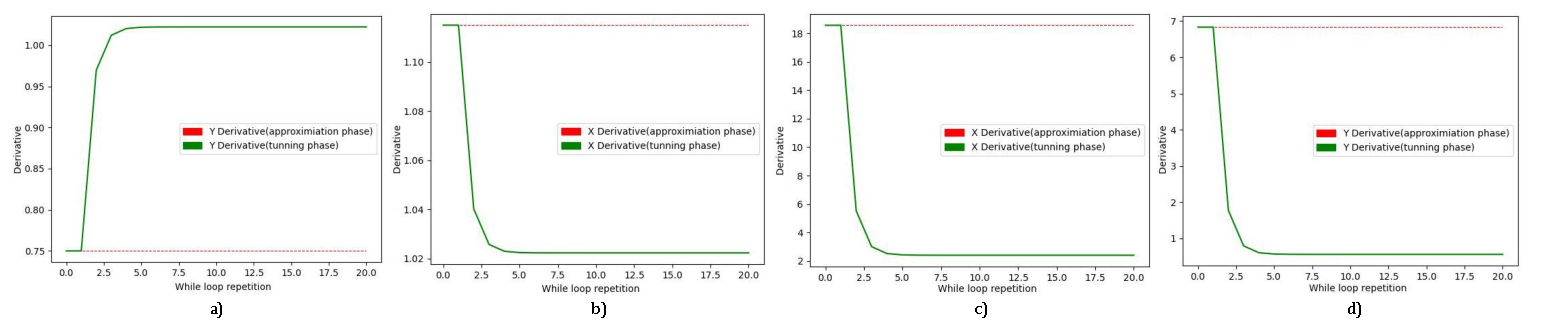
\includegraphics[width=\textwidth]{figures/charts.pdf}
	\caption{Estimated derivative for $e^{(x+y)}$ function from: a) the proposed method I for the noise-free scenario, b) the proposed method III for the noise-free scenario, c) the proposed method I for the noisy version of this function in the original point $(0,0)$, and d) the proposed method III for the noisy version of this function in the original point $(0,0)$.}
	\label{3D_cur23}
\end{figure}

The derivative at the reference point $(0,0)$ is first computed using the proposed methods prior to any parameter tuning. The results for the noise-free case are presented in Fig.~\ref{3D_cur23}(a) and (b). As observed, both methods exhibit fast convergence toward the exact derivative value, indicating the correctness of the underlying mathematical formulation.
\FloatBarrier

To further evaluate robustness, Gaussian noise with a signal-to-noise ratio (SNR) of 10 dB is added to the synthetic function. The corresponding results are shown in Fig.~\ref{3D_cur23}(c) and (d). Despite the presence of noise, the proposed methods are still able to approximate the true derivative with high accuracy, demonstrating strong robustness against noise perturbations.

From a theoretical perspective, it is expected that Methods II and III provide improved performance in noisy conditions compared to Method I, due to their enhanced formulation. In particular, Method III is anticipated to be more robust against impulsive disturbances and outliers, such as salt-and-pepper noise.

%------------------------------------------------
\FloatBarrier
\subsection{Parameter Analysis of the Proposed Methods}

This section evaluates the effects of the neighborhood sample count $n$ and
sample spacing $h$ on the direct squared-loss, iterative squared-loss, and
correntropy gradient estimators. The implementation applies a separable
one-dimensional Taylor approximation independently along the horizontal and
vertical axes, with polynomial order $p=3$. The parameter $n$ denotes the
number of symmetric samples per axis, whereas $h$ specifies the distance
between successive samples. All gradient RMSE and HOG metrics are computed
relative to the clean output obtained with the same estimator and parameter
setting. They therefore measure \emph{noise stability}, rather than absolute
derivative accuracy. Gaussian noise at 20~dB is reported as the
representative distributed-noise condition. Clean matched-self rows are
omitted because they trivially give RMSE $=0$, HOG error $=0$, and cosine
similarity $=1$.

\textbf{Influence of the sample count.}
The $n$ sensitivity experiment fixes $h=1$ and evaluates
$n\in\{4,8,16,32\}$. Increasing $n$ substantially reduces gradient RMSE for
all three methods. Under Gaussian noise at 20~dB, for example, the direct
squared-loss RMSE decreases from 7.077 at $n=4$ to 0.302 at $n=32$.
Nevertheless, the HOG relative error does not improve monotonically: for the
same method it changes from 0.3527 at $n=8$ to 0.3671 at $n=32$. Thus, a
larger support improves gradient-magnitude stability but may reduce spatial
locality and alter the orientation distribution used by HOG.

Under salt-and-pepper noise, correntropy benefits markedly from larger
neighborhoods. At 5\% noise and $n=16$, it reduces RMSE from 4.686 to 2.262
and HOG relative error from 0.5535 to 0.2526 relative to direct squared loss,
while increasing cosine similarity from 0.8468 to 0.9681. At $n=32$, the
corresponding correntropy values improve to 0.899, 0.2027, and 0.9795.
A similar advantage is observed at 10\% noise. The identical direct and
correntropy results observed in several $n=4$ cases should be interpreted
carefully: with $p=3$ and only four samples, the system has limited redundancy
for robust reweighting.

\begin{figure}[H]
	\centering
	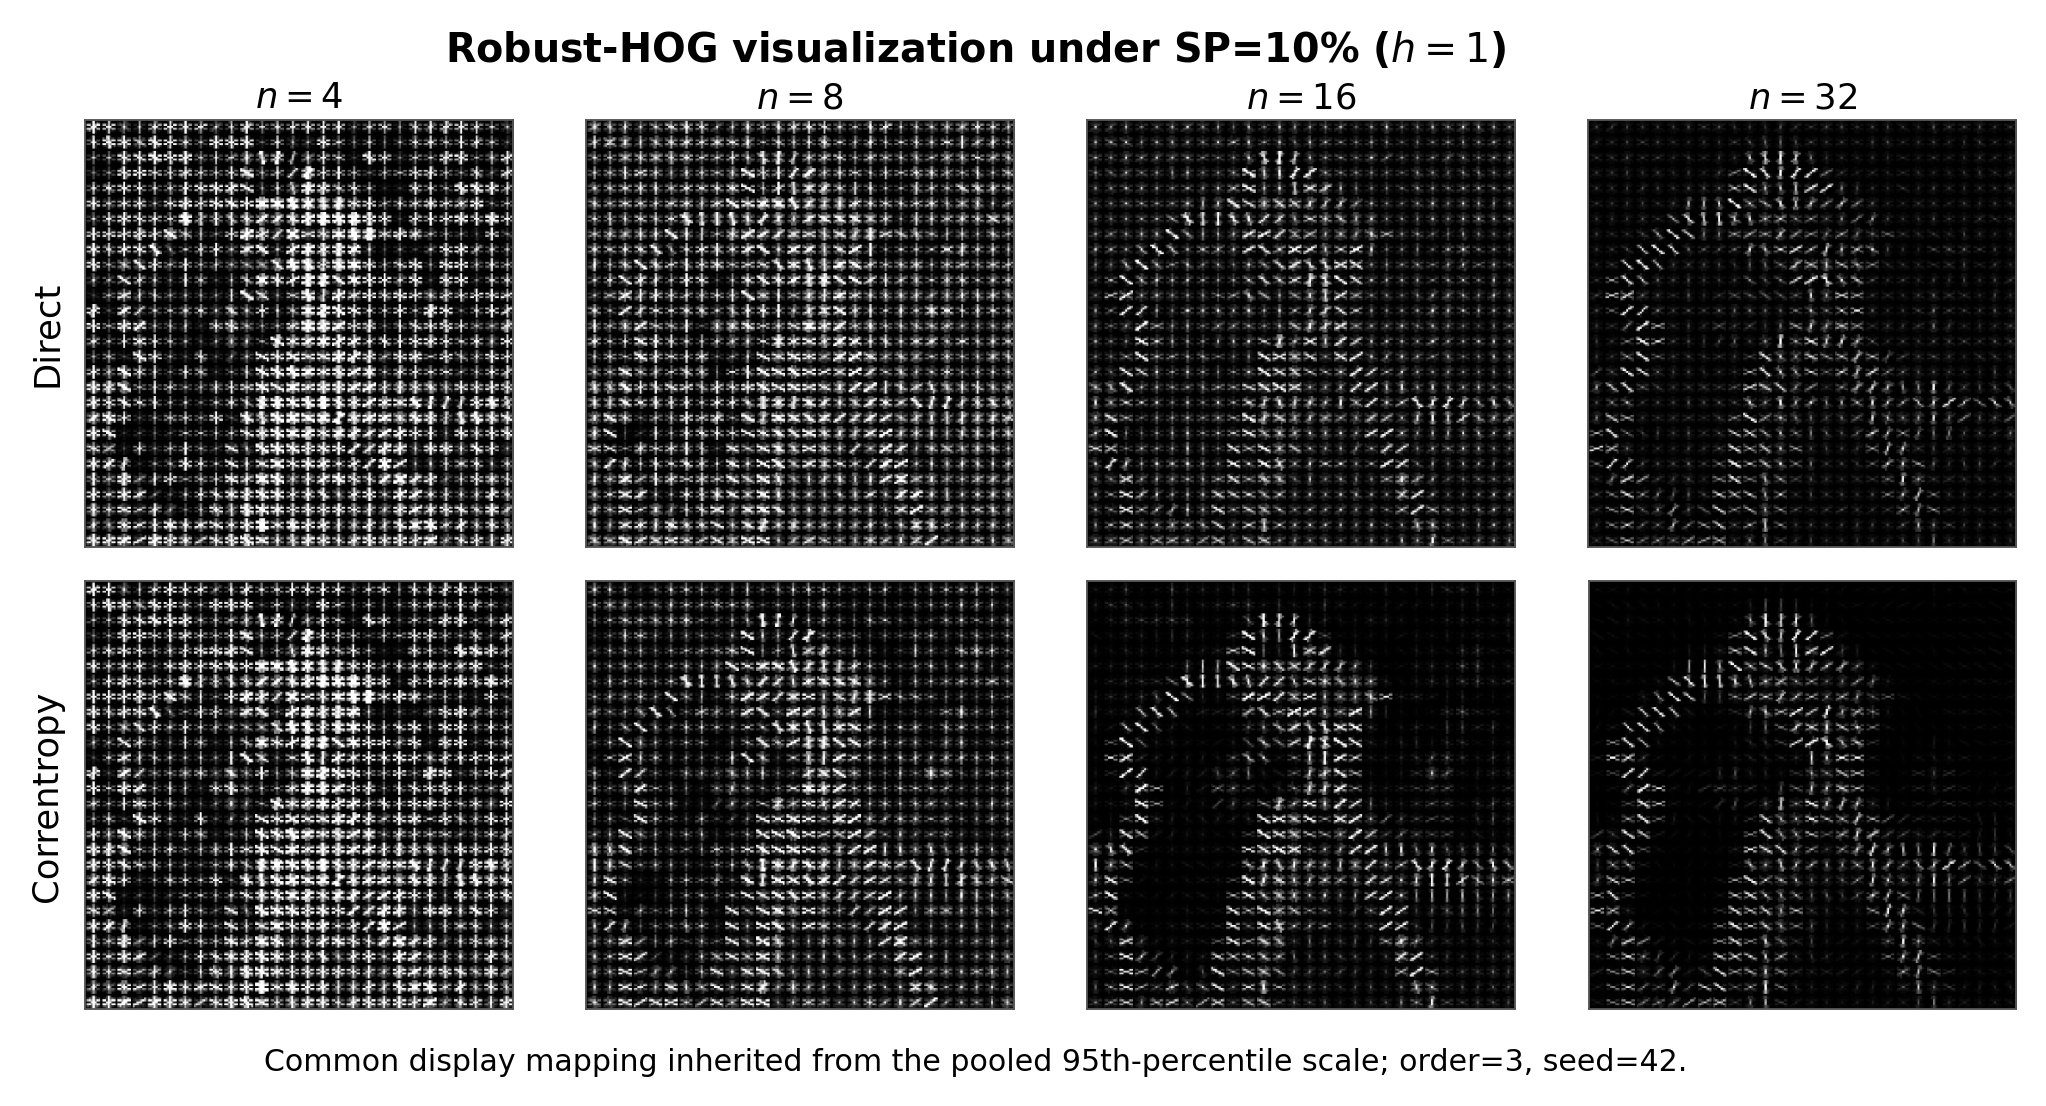
\includegraphics[width=0.96\linewidth]{figures/n_visual_comparison.png}
	\caption{Qualitative Robust-HOG comparison under 10\% salt-and-pepper noise
		for different values of $n$, with $h=1$ and $p=3$.}
	\label{fig:n-visual-comparison}
\end{figure}

\textbf{Influence of sample spacing.}
The $h$ sensitivity experiment fixes $n=8$ and evaluates
$h\in\{1,2,3,4\}$. Under Gaussian noise, increasing $h$ reduces gradient
RMSE but slightly degrades the HOG metrics. For direct squared loss, RMSE
decreases from 2.413 at $h=1$ to 0.573 at $h=4$, whereas HOG relative error
increases from 0.3527 to 0.3896. This indicates stronger smoothing without a
corresponding improvement in descriptor stability.

The opposite tendency is observed under impulsive noise. At 5\%
salt-and-pepper noise, increasing the correntropy spacing from $h=1$ to $h=4$
reduces RMSE from 8.196 to 2.288, reduces HOG relative error from 0.4762 to
0.4120, and increases cosine similarity from 0.8866 to 0.9151. Similar
improvements occur at 10\% noise. Hence, $h=4$ provides the strongest tested
stability under salt-and-pepper noise, although it is the boundary of the
evaluated range and is not claimed to be globally optimal.

\begin{figure}[H]
	\centering
	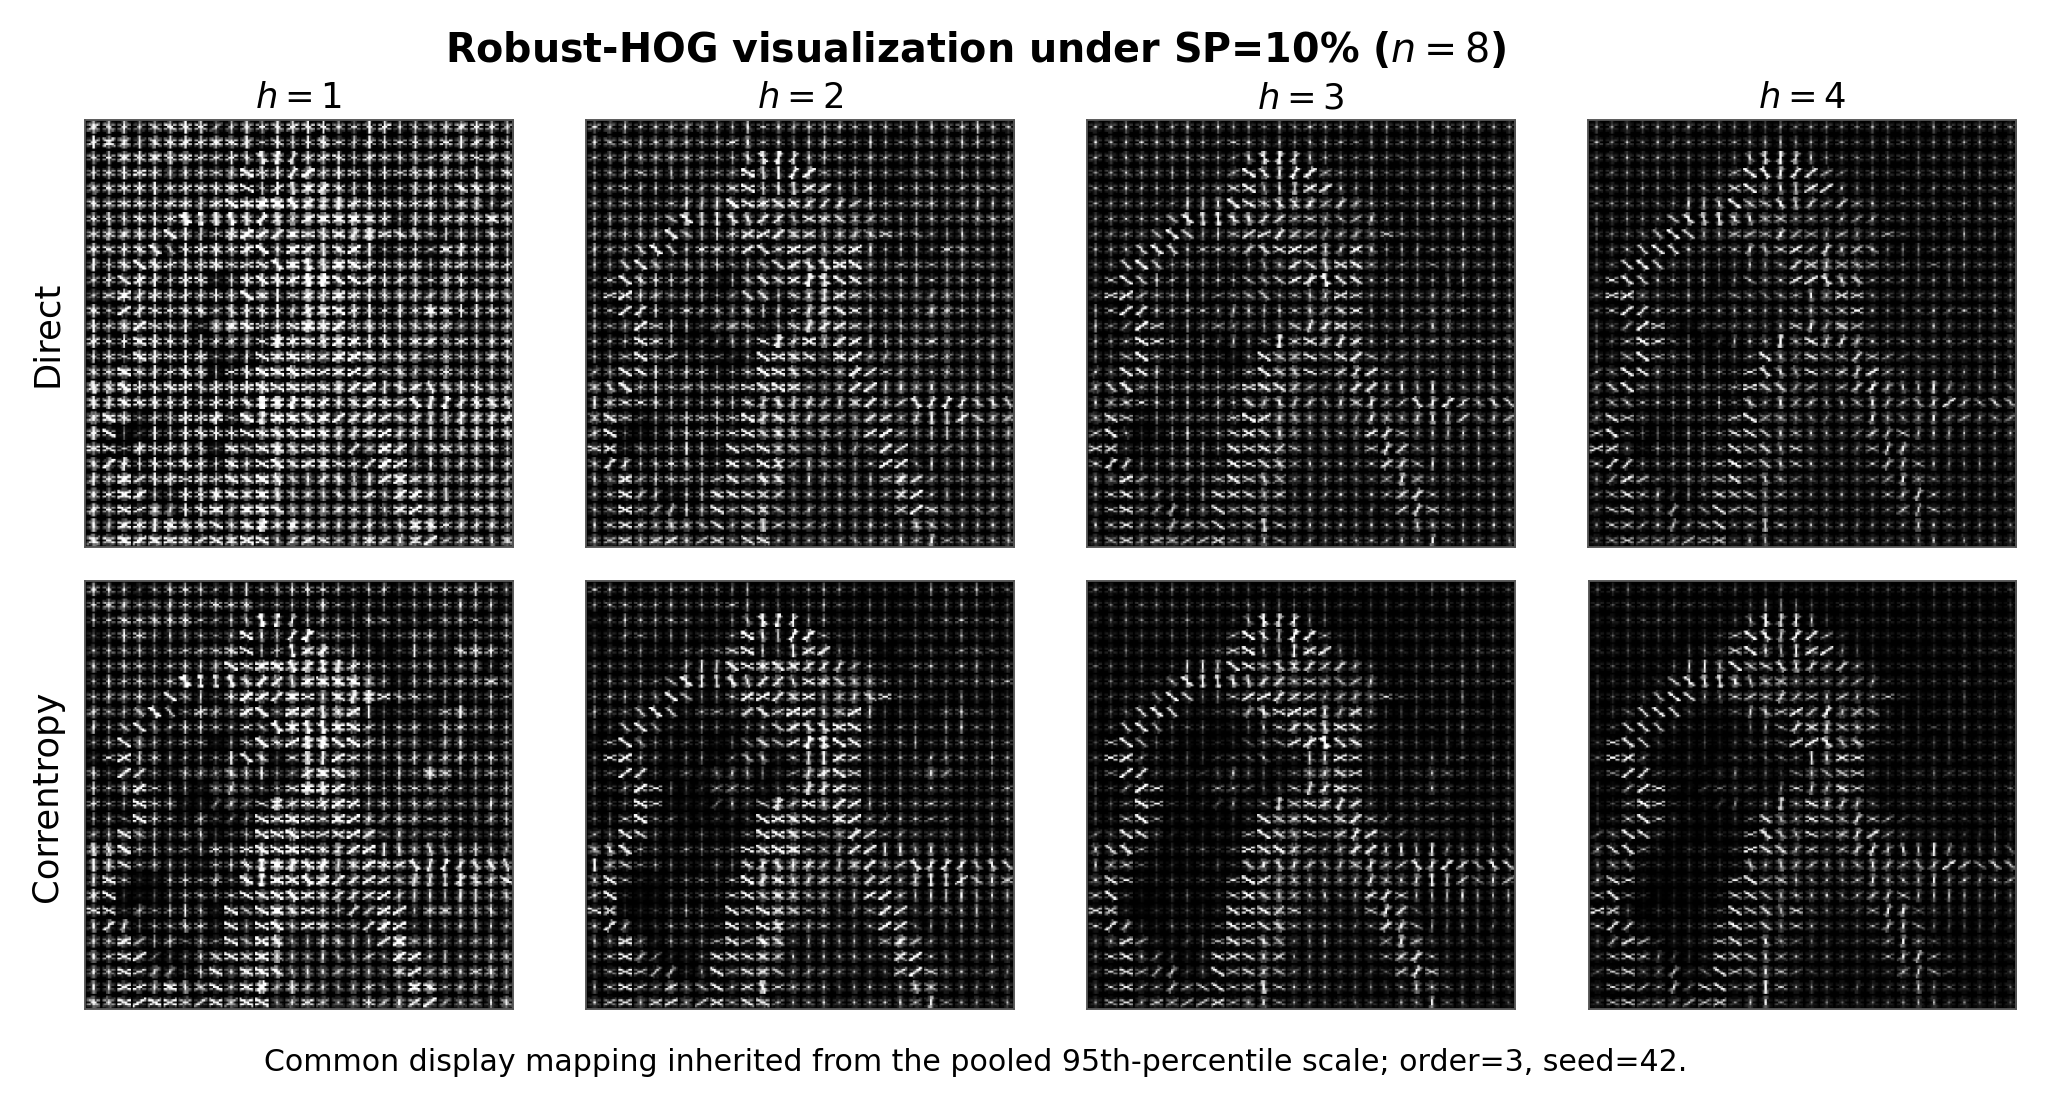
\includegraphics[width=0.96\linewidth]{figures/h_visual_comparison.png}
	\caption{Qualitative Robust-HOG comparison under 10\% salt-and-pepper noise
		for different values of $h$, with $n=8$ and $p=3$.}
	\label{fig:h-visual-comparison}
\end{figure}

\textbf{Comparison of the three estimators.}
The matched-setting tables report results for Gaussian noise at 20~dB and
salt-and-pepper noise at 5\% and 10\%. Gaussian 20~dB is
used as the representative distributed-noise condition. Within each noise
and parameter setting, the three estimators are listed consecutively and use
the same image, region of interest, HOG settings, and seed-42 noise
realization. Clean matched-self rows are omitted because they trivially give
RMSE $=0$, HOG error $=0$, and cosine similarity $=1$.

The direct and iterative squared-loss methods produce almost identical HOG
metrics, while the iterative implementation is consistently several times
slower. For instance, at $n=16$ under 10\% salt-and-pepper noise, their
runtimes are 0.245~s and 0.990~s, although their HOG relative errors are
0.5896 and 0.5899. The iterative method therefore provides no substantial
practical advantage in the present experiments.

Under the representative Gaussian 20~dB condition, the squared-loss
estimators are generally slightly more accurate and considerably faster than
correntropy. At $n=8$ and $h=1$, their RMSE values are 2.413, 2.342, and
3.023 for the direct, iterative, and correntropy methods, respectively. In
contrast, correntropy provides a clear advantage under salt-and-pepper noise,
particularly for $n=16$ and $n=32$. Its benefit should therefore be
interpreted as robustness to impulsive outliers rather than universal
superiority across noise models.

\textbf{Computational cost.}
Figure~\ref{fig:runtime-scaling} reports the median runtime of the complete
gradient-plus-HOG pipeline. The direct estimator is consistently fastest,
followed by the iterative squared-loss method, while correntropy is
substantially more expensive because of its repeated data-dependent
reweighting. For a $256\times256$ image with $n=32$, the measured runtimes
are 0.328~s, 1.641~s, and 28.081~s for the direct, iterative, and correntropy
methods, respectively. Correntropy runtime also depends on convergence
behavior and is therefore not expected to vary strictly monotonically with
$n$.

\begin{figure}[H]
	\centering
	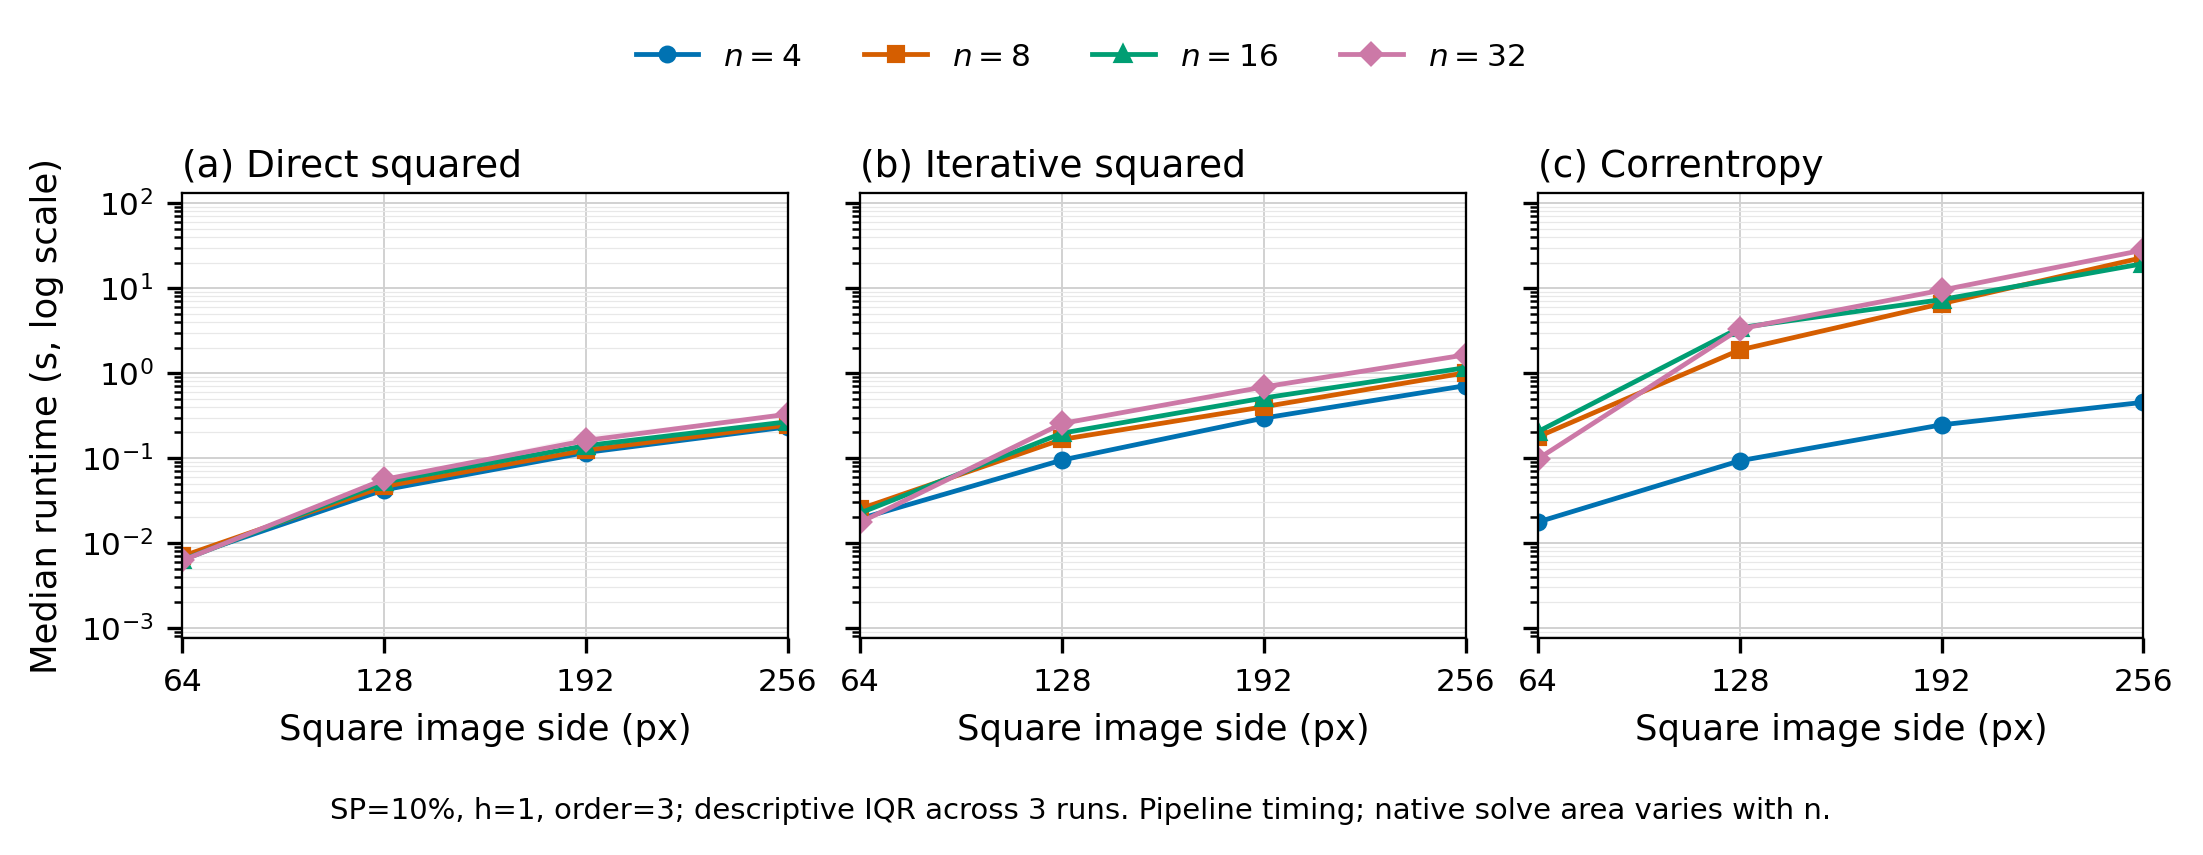
\includegraphics[width=0.94\linewidth]{figures/runtime_scaling_2d.png}
	\caption{Median gradient-plus-HOG runtime under 10\% salt-and-pepper noise
		for $h=1$ and $p=3$. The shared vertical axis is logarithmic, and shaded
		regions show interquartile ranges over three repetitions.}
	\label{fig:runtime-scaling}
\end{figure}

\FloatBarrier
\textbf{Recommended configurations.}
The results indicate that no single configuration is optimal for all noise
models and computational constraints. Direct squared loss with $n=4$ or
$n=8$ is the preferred efficiency-oriented configuration and remains
competitive under Gaussian noise. The iterative squared-loss method produces
similar quality at higher computational cost and is therefore retained mainly
as an optimization baseline. Among the measured correntropy candidates,
$(n,h)=(16,4)$ provides the most practical balance between impulsive-noise
stability and runtime, whereas $(n,h)=(32,1)$ provides the strongest measured
robustness at substantially higher cost.

Overall, squared loss is preferable for Gaussian noise and
runtime-constrained applications, whereas correntropy is preferable when
robustness to salt-and-pepper noise is the primary requirement. These
conclusions are based on one source image and seed 42. Moreover, the $n$ and
$h$ studies are one-factor-at-a-time experiments; therefore, no unmeasured
combination, including $(32,4)$, is claimed to be optimal.



%------------------------------------------------
\FloatBarrier
\subsection{Comparison with Sobel and Robustness Evaluation}
To assess the practical effectiveness of the proposed gradient estimators,
their resulting HOG representations are compared with those obtained using
the conventional Sobel operator. The comparison is designed to examine two
complementary properties: preservation of the underlying image structure
under noise-free conditions and stability of the extracted descriptor in
the presence of distributed and impulsive disturbances. For a fair
comparison, all methods are applied to the same input images and use an
identical HOG configuration, while only the gradient-estimation stage is
changed. Methods~I, II, and III respectively denote the direct squared-loss,
iterative squared-loss, and correntropy-based formulations introduced in
Section~\ref{sec:proposed-method}. The experiments include four images with
different structural characteristics, comprising object contours, curved
boundaries, textured regions, and architectural edges.

Table~\ref{tab:sobel-clean-comparison} first presents the results obtained
from the original noise-free images. This experiment serves as a reference
case for determining whether the increased robustness of the proposed
estimators is achieved without distorting the principal gradient
orientations under ideal conditions. Since no artificial degradation is
introduced in this setting, large differences among the methods are not
expected; instead, the objective is to verify that the proposed formulations
preserve the main edge and orientation structures represented by
Sobel-based HOG.
%------------------------------------------------
\FloatBarrier
\begin{table}[!h]
\centering
\caption{Performance evaluation, for the proposed methods I, II, and III (with $h=1$ and $n=32$) and other compared method, i.e., Sobel over four images without noise}
\label{tab1}
\begin{adjustbox}{width=10cm,height=3.25cm}

\begin{tabular}{l|l|l|l|l}
\hline \hline
\begin{tabular}[c]{@{}l@{}}Original clean\\ image\end{tabular}
& 
\includegraphics[width=0.5in,height=0.5in]{figures/cameraman.png}  
& 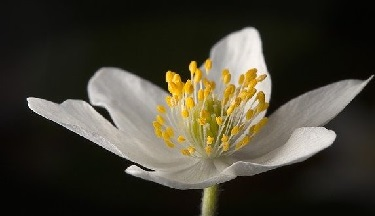
\includegraphics[width=0.5in,height=0.5in]{figures/flower.jpg}
& 
\includegraphics[width=0.5in,height=0.5in]{figures/girl.png}
& 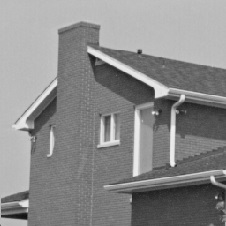
\includegraphics[width=0.5in,height=0.5in]{figures/home.jpg}
\\ \hline

\begin{tabular}[c]{@{}l@{}}Proposed Method I\end{tabular} 
& 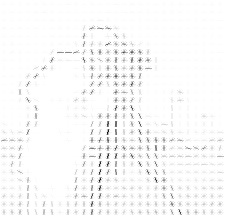
\includegraphics[width=0.5in,height=0.5in]{second_table_n0_s1/cnoise_0.jpg}
& 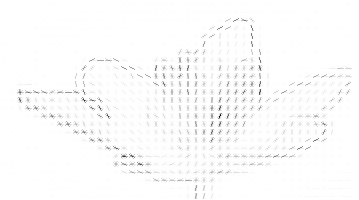
\includegraphics[width=0.5in,height=0.5in]{second_table_n0_s1/fnoise_0.jpg}
& 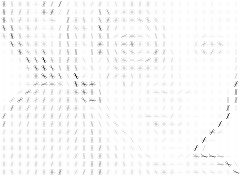
\includegraphics[width=0.5in,height=0.5in]{second_table_n0_s1/gnoise_0.jpg}
& 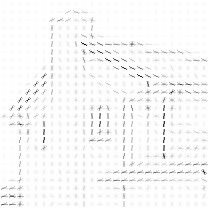
\includegraphics[width=0.5in,height=0.5in]{second_table_n0_s1/hnoise_0.jpg}
\\ \hline

\begin{tabular}[c]{@{}l@{}}Proposed Method II\end{tabular} 
& 
\includegraphics[width=0.5in,height=0.5in]{second_table_n0_s2/cnoise_0.jpg}
& 
\includegraphics[width=0.5in,height=0.5in]{second_table_n0_s2/fnoise_0.jpg} 
& 
\includegraphics[width=0.5in,height=0.5in]{second_table_n0_s2/gnoise_0.jpg}% size?
& 
\includegraphics[width=0.5in,height=0.5in]{second_table_n0_s2/hnoise_0.jpg}
\\ \hline
%done%done%done%done%done
\begin{tabular}[c]{@{}l@{}}Proposed Method III\end{tabular} 
& 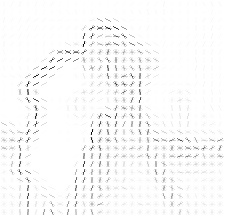
\includegraphics[width=0.5in,height=0.5in]{second_table_n0_s3/cnoise_50.jpg}
& 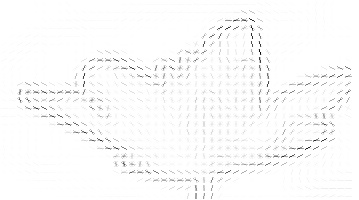
\includegraphics[width=0.5in,height=0.5in]{second_table_n0_s3/fnoise_50.jpg}
& 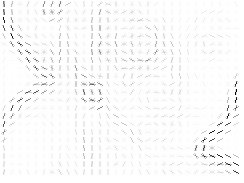
\includegraphics[width=0.5in,height=0.5in]{second_table_n0_s3/gnoise_50.jpg}
& 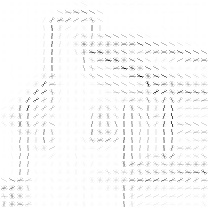
\includegraphics[width=0.5in,height=0.5in]{second_table_n0_s3/hnoise_50.jpg}
\\ \hline

Sobel method
      & 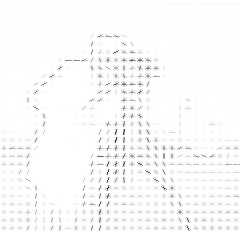
\includegraphics[width=0.5in,height=0.5in]{second_table_sobel_n0/cnoise.jpg}
& 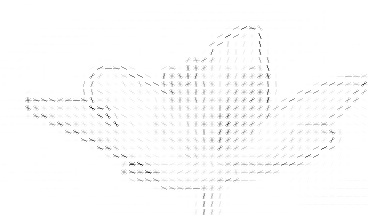
\includegraphics[width=0.5in,height=0.5in]{second_table_sobel_n0/fnoise.jpg}
& 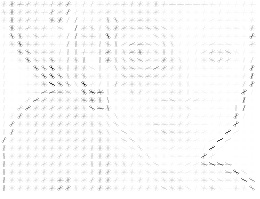
\includegraphics[width=0.5in,height=0.5in]{second_table_sobel_n0/gnoise.jpg}
& 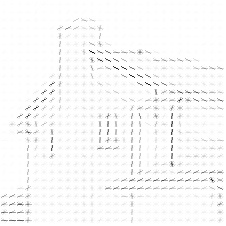
\includegraphics[width=0.5in,height=0.5in]{second_table_sobel_n0/hnoise.jpg}
\\ \hline \hline
\end{tabular}
\end{adjustbox}
\end{table}
%------------------------------------------------
Table~\ref{tab:sobel-gaussian-comparison} subsequently evaluates the methods
under Gaussian noise. This experiment examines their response to a
distributed perturbation that affects the image over the entire spatial
domain. The purpose is to determine whether the proposed local polynomial
estimators can reduce descriptor distortion while retaining relevant edge
orientations, rather than to assume that the robust correntropy formulation
must necessarily dominate the squared-loss alternatives for Gaussian
contamination.

\FloatBarrier
\begin{table}[!h]
\centering
\caption{Performance evaluation, for the proposed methods I, II, and III (with $h=1$ and $n=32$, respectively) and other compared method, i.e., Sobel over four images contaminated by Gaussian noise with 50$dB$ power}
\label{tab2}
\begin{adjustbox}{width=10cm,height=3.25cm}

\begin{tabular}{l|l|l|l|l}
\hline \hline
\begin{tabular}[c]{@{}l@{}}Noisy image\end{tabular}
    &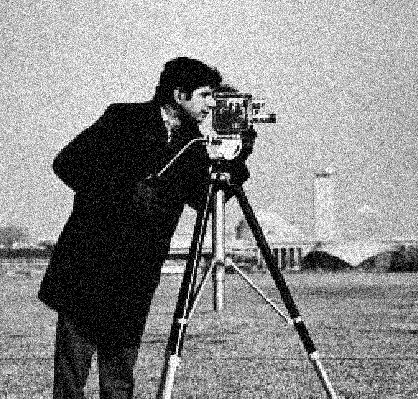
\includegraphics[width=0.5in,height=0.5in]{figures/cameraman_gaussian.jpg}
    &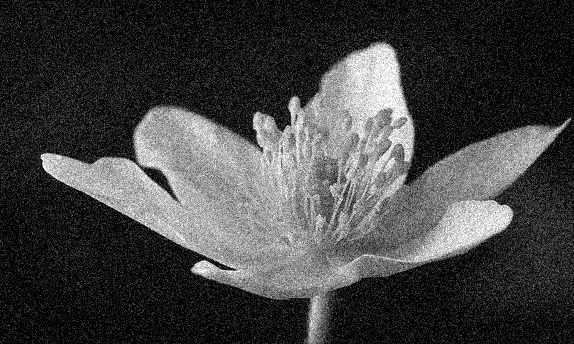
\includegraphics[width=0.5in,height=0.5in]{figures/flower_gussian.jpg}
    &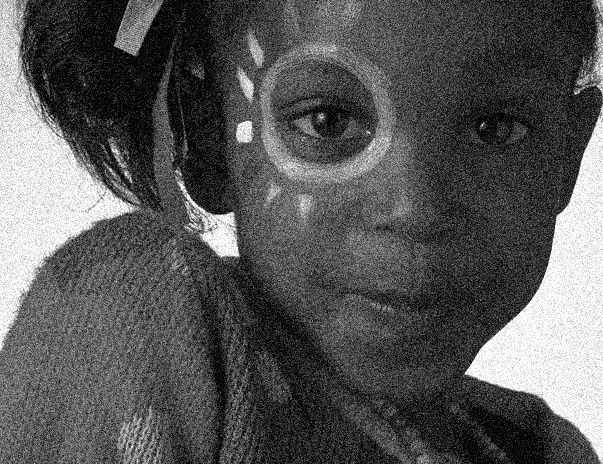
\includegraphics[width=0.5in,height=0.5in]{figures/girl_gaussian.jpg}
    &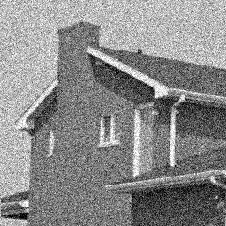
\includegraphics[width=0.5in,height=0.5in]{figures/home_gaussian2.jpg}
\\ \hline
            
\begin{tabular}[c]{@{}l@{}}Proposed Method I\end{tabular} 
& 
\includegraphics[width=0.5in,height=0.5in]{second_table_n50_s1/cnoise_50.jpg}
& 
\includegraphics[width=0.5in,height=0.5in]{second_table_n50_s1/fnoise_50.jpg}
& 
\includegraphics[width=0.5in,height=0.5in]{second_table_n50_s1/gnoise_50.jpg}
& 
\includegraphics[width=0.5in,height=0.5in]{second_table_n50_s1/hnoise_50.jpg}
\\ \hline

\begin{tabular}[c]{@{}l@{}}Proposed Method II\end{tabular} 
& 
\includegraphics[width=0.5in,height=0.5in]{second_table_n50_s2/cnoise_50.jpg}
& 
\includegraphics[width=0.5in,height=0.5in]{second_table_n50_s2/fnoise_50.jpg} 
& 
\includegraphics[width=0.5in,height=0.5in]{second_table_n50_s2/gnoise_50.jpg}% size?
& 
\includegraphics[width=0.5in,height=0.5in]{second_table_n50_s2/hnoise_50.jpg}
\\ \hline
%done%done%done%done%done
\begin{tabular}[c]{@{}l@{}}Proposed Method III\end{tabular} 
& 
\includegraphics[width=0.5in,height=0.5in]{second_table_n50_s3/cnoise_50.jpg}
& 
\includegraphics[width=0.5in,height=0.5in]{second_table_n50_s3/fnoise_50.jpg}
& 
\includegraphics[width=0.5in,height=0.5in]{second_table_n50_s3/gnoise_50.jpg}
& 
\includegraphics[width=0.5in,height=0.5in]{second_table_n50_s3/hnoise_50.jpg}
\\ \hline

Sobel method
& 
\includegraphics[width=0.5in,height=0.5in]{second_table_sobel_n50/cnoise_50.jpg}
& 
\includegraphics[width=0.5in,height=0.5in]{second_table_sobel_n50/fnoise_50.jpg}
& 
\includegraphics[width=0.5in,height=0.5in]{second_table_sobel_n50/gnoise_50.jpg}
& 
\includegraphics[width=0.5in,height=0.5in]{second_table_sobel_n50/hnoise_50.jpg}
\\ \hline \hline        
\end{tabular}
\end{adjustbox}
\end{table}
%------------------------------------------------
Finally, Table~\ref{tab:sobel-sp-comparison} reports the results under
salt-and-pepper noise. This scenario provides the principal robustness test,
because isolated high-amplitude pixels produce strong and potentially
misleading responses in conventional finite-difference gradients. The
comparison is therefore intended to show whether the proposed methods, and
particularly the correntropy-based Method~III, suppress impulsive responses
more effectively while preserving the dominant structural orientations of
the original images.

\FloatBarrier
\begin{table}[!th]
\centering
\caption{Performance evaluation, for the proposed methods I, II, and III (with $h=1$ and $n=32$) and other compared method, i.e., Sobel over four images contaminated by 5$\%$ salt and pepper noise }
\label{tab3}
\begin{adjustbox}{width=10cm,height=3.25cm}

\begin{tabular}{l|l|l|l|l}
\hline \hline    
\begin{tabular}[c]{@{}l@{}}Noisy image\end{tabular}
    &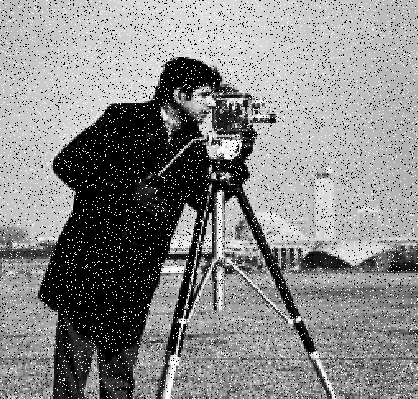
\includegraphics[width=0.5in,height=0.5in]{figures/cameraman_saltpaper.png}
    &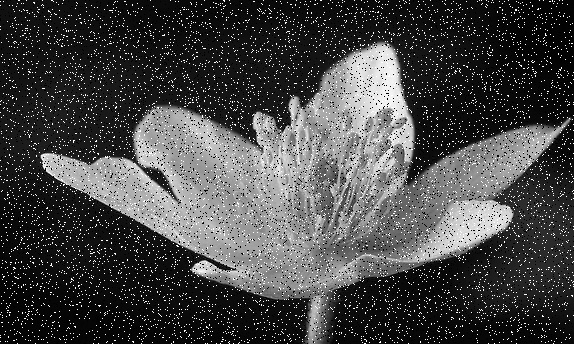
\includegraphics[width=0.5in,height=0.5in]{figures/flower_saltpaper.jpg}   &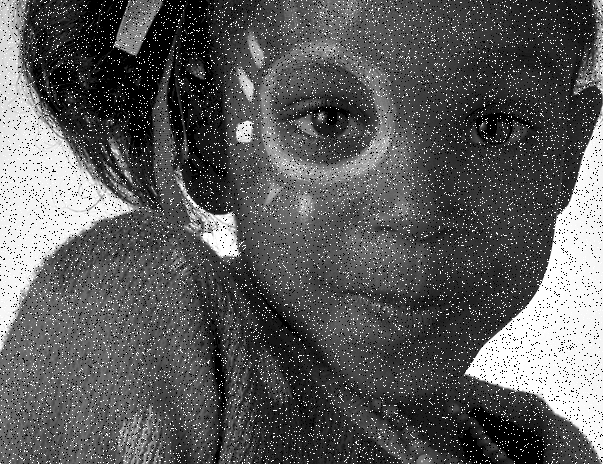
\includegraphics[width=0.5in,height=0.5in]{figures/girl_saltpaper.png}
    &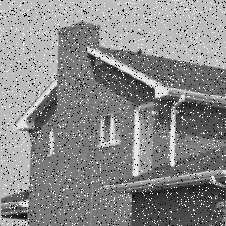
\includegraphics[width=0.5in,height=0.5in]{figures/home_saltpaper_5.png}
\\ \hline

\begin{tabular}[c]{@{}l@{}}Proposed Method I\end{tabular} 
& 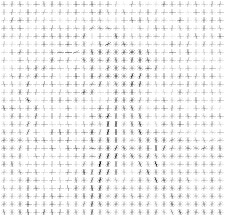
\includegraphics[width=0.5in,height=0.5in]{second_table_n5_s1/cnoise_5.jpg}
& 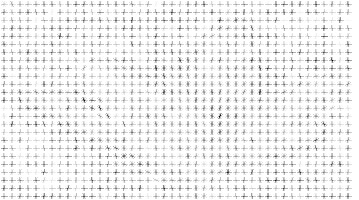
\includegraphics[width=0.5in,height=0.5in]{second_table_n5_s1/fnoise_5.jpg}
& 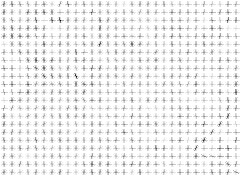
\includegraphics[width=0.5in,height=0.5in]{second_table_n5_s1/gnoise_5.jpg}
& 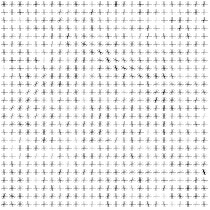
\includegraphics[width=0.5in,height=0.5in]{second_table_n5_s1/hnoise_5.jpg}
\\ \hline   

\begin{tabular}[c]{@{}l@{}}Proposed Method II\end{tabular} 
& 
\includegraphics[width=0.5in,height=0.5in]{second_table_n5_s2/cnoise_5.jpg}
& 
\includegraphics[width=0.5in,height=0.5in]{second_table_n5_s2/fnoise_5.jpg} 
& 
\includegraphics[width=0.5in,height=0.5in]{second_table_n5_s2/gnoise_5.jpg}% size?
& 
\includegraphics[width=0.5in,height=0.5in]{second_table_n5_s2/hnoise_5.jpg}
\\ \hline
%done%done%done%done%done
\begin{tabular}[c]{@{}l@{}}Proposed Method III\end{tabular} 
& 
\includegraphics[width=0.5in,height=0.5in]{second_table_n5_s3/cnoise_5.jpg}
& 
\includegraphics[width=0.5in,height=0.5in]{second_table_n5_s3/fnoise_5.jpg}
& 
\includegraphics[width=0.5in,height=0.5in]{second_table_n5_s3/gnoise_5.jpg}
& 
\includegraphics[width=0.5in,height=0.5in]{second_table_n5_s3/hnoise_5.jpg}
\\ \hline

Sobel method
& 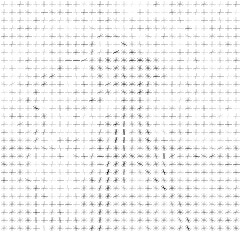
\includegraphics[width=0.5in,height=0.5in]{second_table_sobel_n5/cnoise_3.jpg}
& 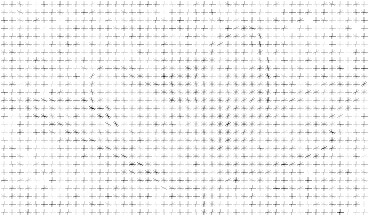
\includegraphics[width=0.5in,height=0.5in]{second_table_sobel_n5/fnoise_3.jpg}
& 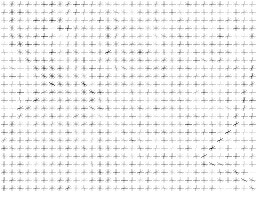
\includegraphics[width=0.5in,height=0.5in]{second_table_sobel_n5/gnoise_3.jpg}
& 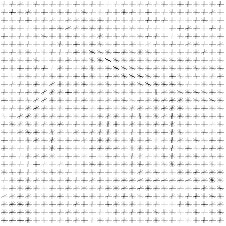
\includegraphics[width=0.5in,height=0.5in]{second_table_sobel_n5/hnoise_3.jpg}
\\ \hline \hline
\end{tabular}
\end{adjustbox}
\end{table}
%------------------------------------------------
\FloatBarrier
Overall, the proposed methods produce HOG representations comparable to Sobel under noise-free conditions, indicating that the modified gradient estimation does not noticeably distort the main image structures. Under
Gaussian noise, they provide cleaner and more stable orientation patterns. The advantage becomes more evident under salt-and-pepper noise, where Method~III better suppresses impulsive responses while preserving the dominant edges. These observations support the improved noise robustness of the proposed estimators, particularly for non-Gaussian contamination.

Figure~\ref{New3} provides a closer view of the HOG responses under 3\%
salt-and-pepper noise. Method~I remains sensitive to impulsive pixels,
leading to irregular orientation responses and weaker preservation of the
dominant diagonal edge. Iterative reweighting in Method~II reduces part of
this disturbance, whereas the correntropy-based Method~III produces the most
coherent orientation pattern and fewer isolated responses. This visual
observation is consistent with the improved robustness of Method~III under
non-Gaussian contamination.
\FloatBarrier
%-------------------------------------------
\begin{figure*}[!th]
	\centering
	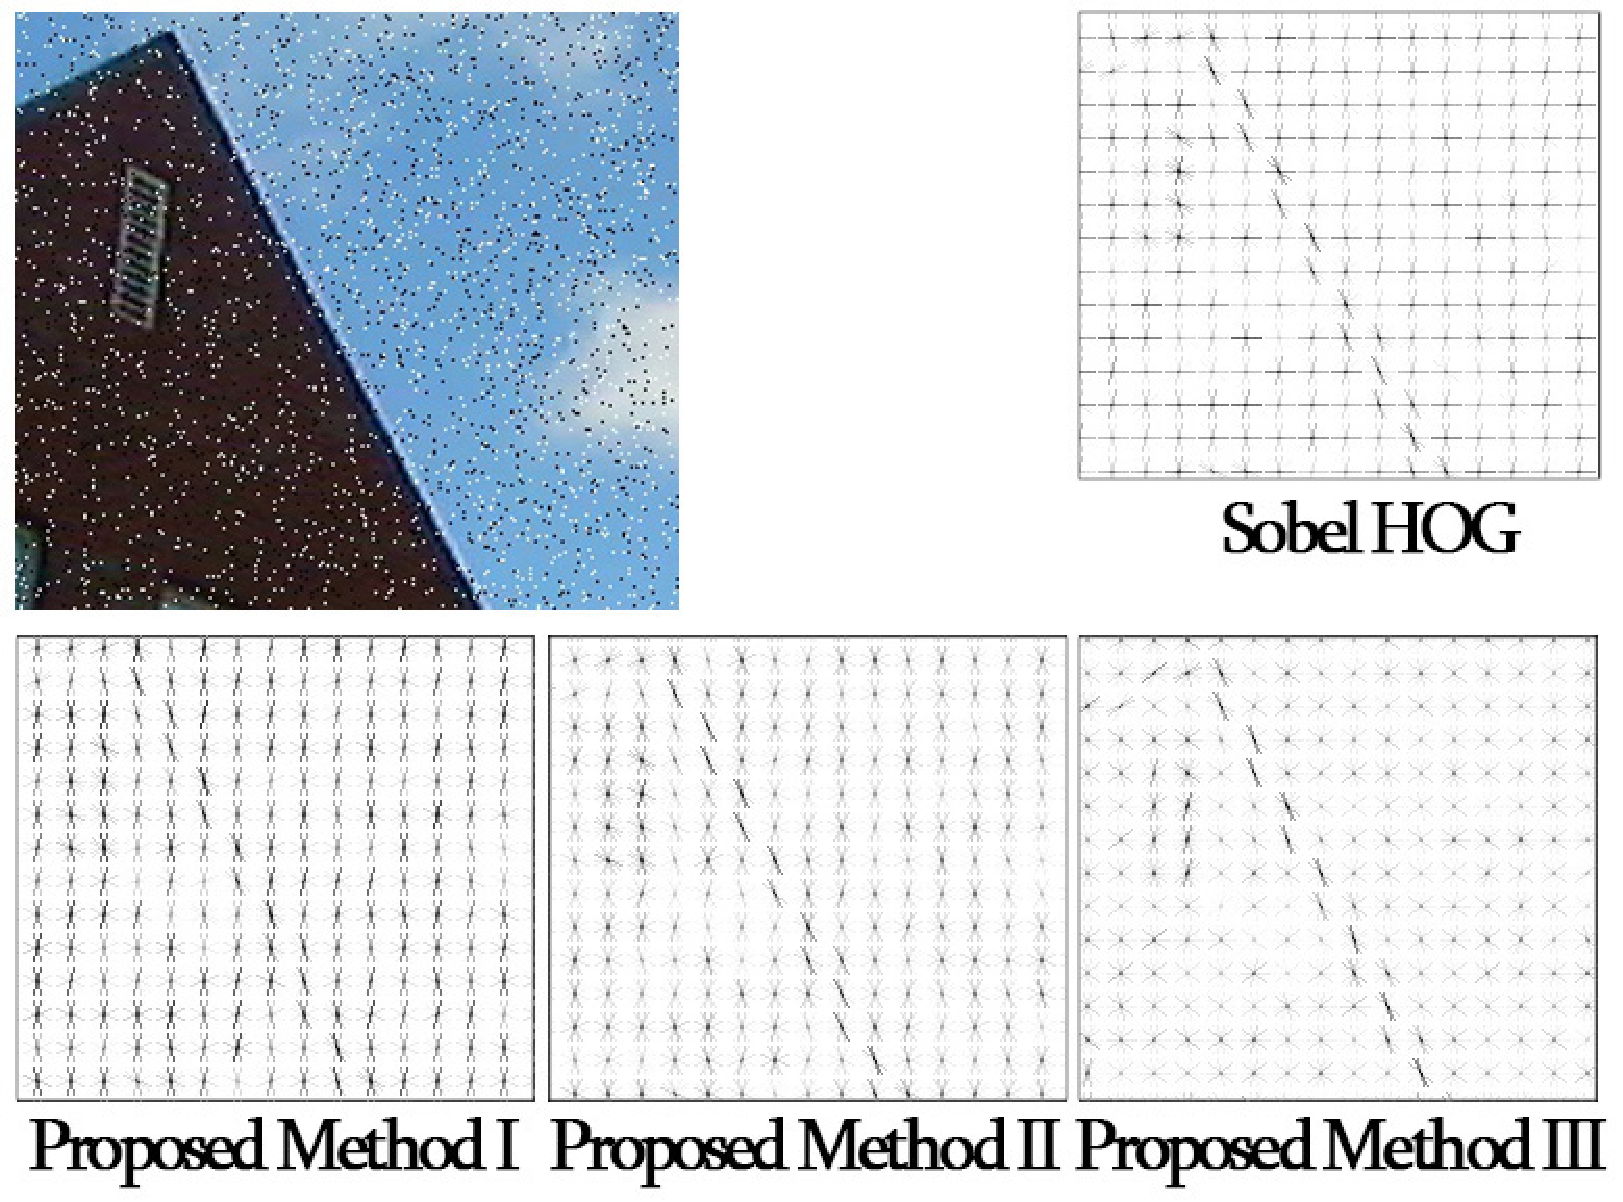
\includegraphics[height=4cm,width=8cm]{comparing_Robustness_of_images.pdf}
	\caption{Detailed comparison of HOG orientation responses under 3\%
	salt-and-pepper noise. Method~III preserves the dominant diagonal structure
	while reducing isolated responses caused by impulsive pixels.}
	\label{New3}
\end{figure*}

\FloatBarrier

\FloatBarrier
\section{Conclusions}

In this work, a robust HOG-based feature extraction framework was proposed by
integrating Taylor-series-based gradient estimation with robust optimization
strategies. Three gradient estimators were developed, including direct
squared-loss, iterative squared-loss, and correntropy-based formulations, to
improve the stability of gradient computation under noisy conditions.

The experimental results demonstrated that the proposed estimators preserve
the main image structures in noise-free conditions while providing improved
stability under noisy observations. In particular, the correntropy-based
formulation showed better resistance to impulsive salt-and-pepper noise by
reducing the influence of outlier pixels, whereas the squared-loss-based
methods provided lower computational complexity.

The effects of the neighborhood parameters, including the sample count $n$
and sampling distance $h$, were also investigated. The results showed that
these parameters introduce a robustness--complexity trade-off, where larger
neighborhoods can improve noise stability at the cost of increased execution
time. The comparison with the conventional Sobel operator further confirmed
that the proposed gradient estimators can provide more stable HOG
representations, especially under challenging noisy conditions.

Overall, the proposed framework provides a flexible approach for robust HOG
feature extraction by combining accurate local gradient approximation with
noise-resistant optimization. Future work will focus on extending the
evaluation to larger-scale datasets and investigating adaptive parameter
selection strategies for different image characteristics and noise models.
%------------------------------------------------

\section*{Reference}
\bibliography{ref}
\end{document}
%------------------------------------------------
